%%%%%%%%%%%%%%%%%%%%%---Chapter5 Formatting---%%%%%%%%%%%%%%%%%%%%%%%%%%%%%%%%%%
\documentclass[Thesis.tex]{subfiles}
\begin{document}
\setcounter{chapter}{4} %%Chapter Numbering


%%%%%%%%%%%%%%%%%%%%%%%%%%%%%%%%%%%%%%%%%%%%%%%%%%%%%%%%%%%%%%%%%%%%%%%%%%%%

\chapter{Results: Error Mitigation Benchmark}\label{chap5:results}

Sections~\ref{sec:ch5_main}--\ref{sec:ch5_summary} evaluate mitigation under
idealised Markovian noise, including bandwidth sensitivity, feature ablations
and depth and circuit-family transfer. Sections~\ref{sec:ch5_nonmarkov}--
\ref{sec:ch5_realistic_summary} use the device-informed model to compare scaling
protocols, test defect and drift controls, and evaluate the accuracy and circuit
cost of finite-shot fidelity kernels.

Unless stated otherwise, error is RMSE against the ideal expectation value.
Negative error reduction indicates higher RMSE than the unmitigated estimator.
Within a fitted split, the $95\%$ bootstrap resamples whole test circuits and
pairs the methods' errors on the same circuits (Section~\ref{sec:ch3_metrics}).
Replications across independently generated pools report nominal intervals over
the paired pool means. A difference is called \emph{resolved} when its paired
interval excludes zero. Appendix~\ref{AppendixB} gives numerical tables and
the files containing the replications.

\section{Main benchmark}\label{sec:ch5_main}

Table~\ref{tab:ch5_main} and Figure~\ref{fig:ch5_main} report all ten arms on
Split~A ($3150$ training rows, $1350$ test rows, grouped by circuit) and Split~B
($2700$ training rows at depth $\leq 4$, $1800$ test rows at depth $\geq 5$).

\begin{table}[htbp]
\centering
\caption[Main benchmark, both splits]{Main benchmark. RMSE against the ideal expectation value with $95\%$
bootstrap confidence intervals; error reduction relative to the unmitigated
estimator on the same fold. Arms are ordered by Split~A error. Negative error
reduction means the method is worse than no mitigation. All values are for the
single reference fit. Section~\ref{sec:ch5_robustness} reports a separate
ten-seed VQC study.}
\label{tab:ch5_main}
\small
\begin{tabular}{llcccc}
\toprule
& & \multicolumn{2}{c}{\textbf{Split A: random circuits}}
  & \multicolumn{2}{c}{\textbf{Split B: deeper circuits}} \\
\cmidrule(lr){3-4} \cmidrule(lr){5-6}
\textbf{Method} & \textbf{Family} & \textbf{RMSE (95\% CI)} & \textbf{Red.\ \%}
& \textbf{RMSE} & \textbf{Red.\ \%} \\
\midrule
Classical RBF kernel ridge & classical & 0.0404 (0.0380--0.0427) & 60.9 & \textbf{0.0658} & \textbf{46.0} \\
Neural net (64,64) & classical & 0.0412 (0.0388--0.0434) & 60.2 & 0.1292 & $-6.2$ \\
Quantum kernel ridge & hybrid & 0.0421 (0.0395--0.0448) & 59.3 & 0.1433 & $-17.7$ \\
Gradient-boosted trees & classical & 0.0436 (0.0413--0.0460) & 57.8 & 0.0665 & 45.4 \\
Ridge regression & classical & 0.0515 (0.0488--0.0543) & 50.2 & 0.0717 & 41.1 \\
Data-reuploading VQC & hybrid & 0.0533 (0.0510--0.0557) & 48.5 & 0.3127 & $-156.8$ \\
ZNE, linear & analytic & 0.0737 (0.0690--0.0785) & 28.8 & 0.0960 & 21.2 \\
ZNE, Richardson (deg 2) & analytic & 0.0743 (0.0713--0.0773) & 28.2 & 0.0831 & 31.8 \\
No mitigation & --- & 0.1035 (0.0978--0.1090) & 0.0 & 0.1217 & 0.0 \\
ZNE, exponential & analytic & 0.1548 (0.1382--0.1714) & $-49.6$ & 0.1805 & $-48.3$ \\
\bottomrule
\end{tabular}
\end{table}

\begin{figure}[htbp]
\centering
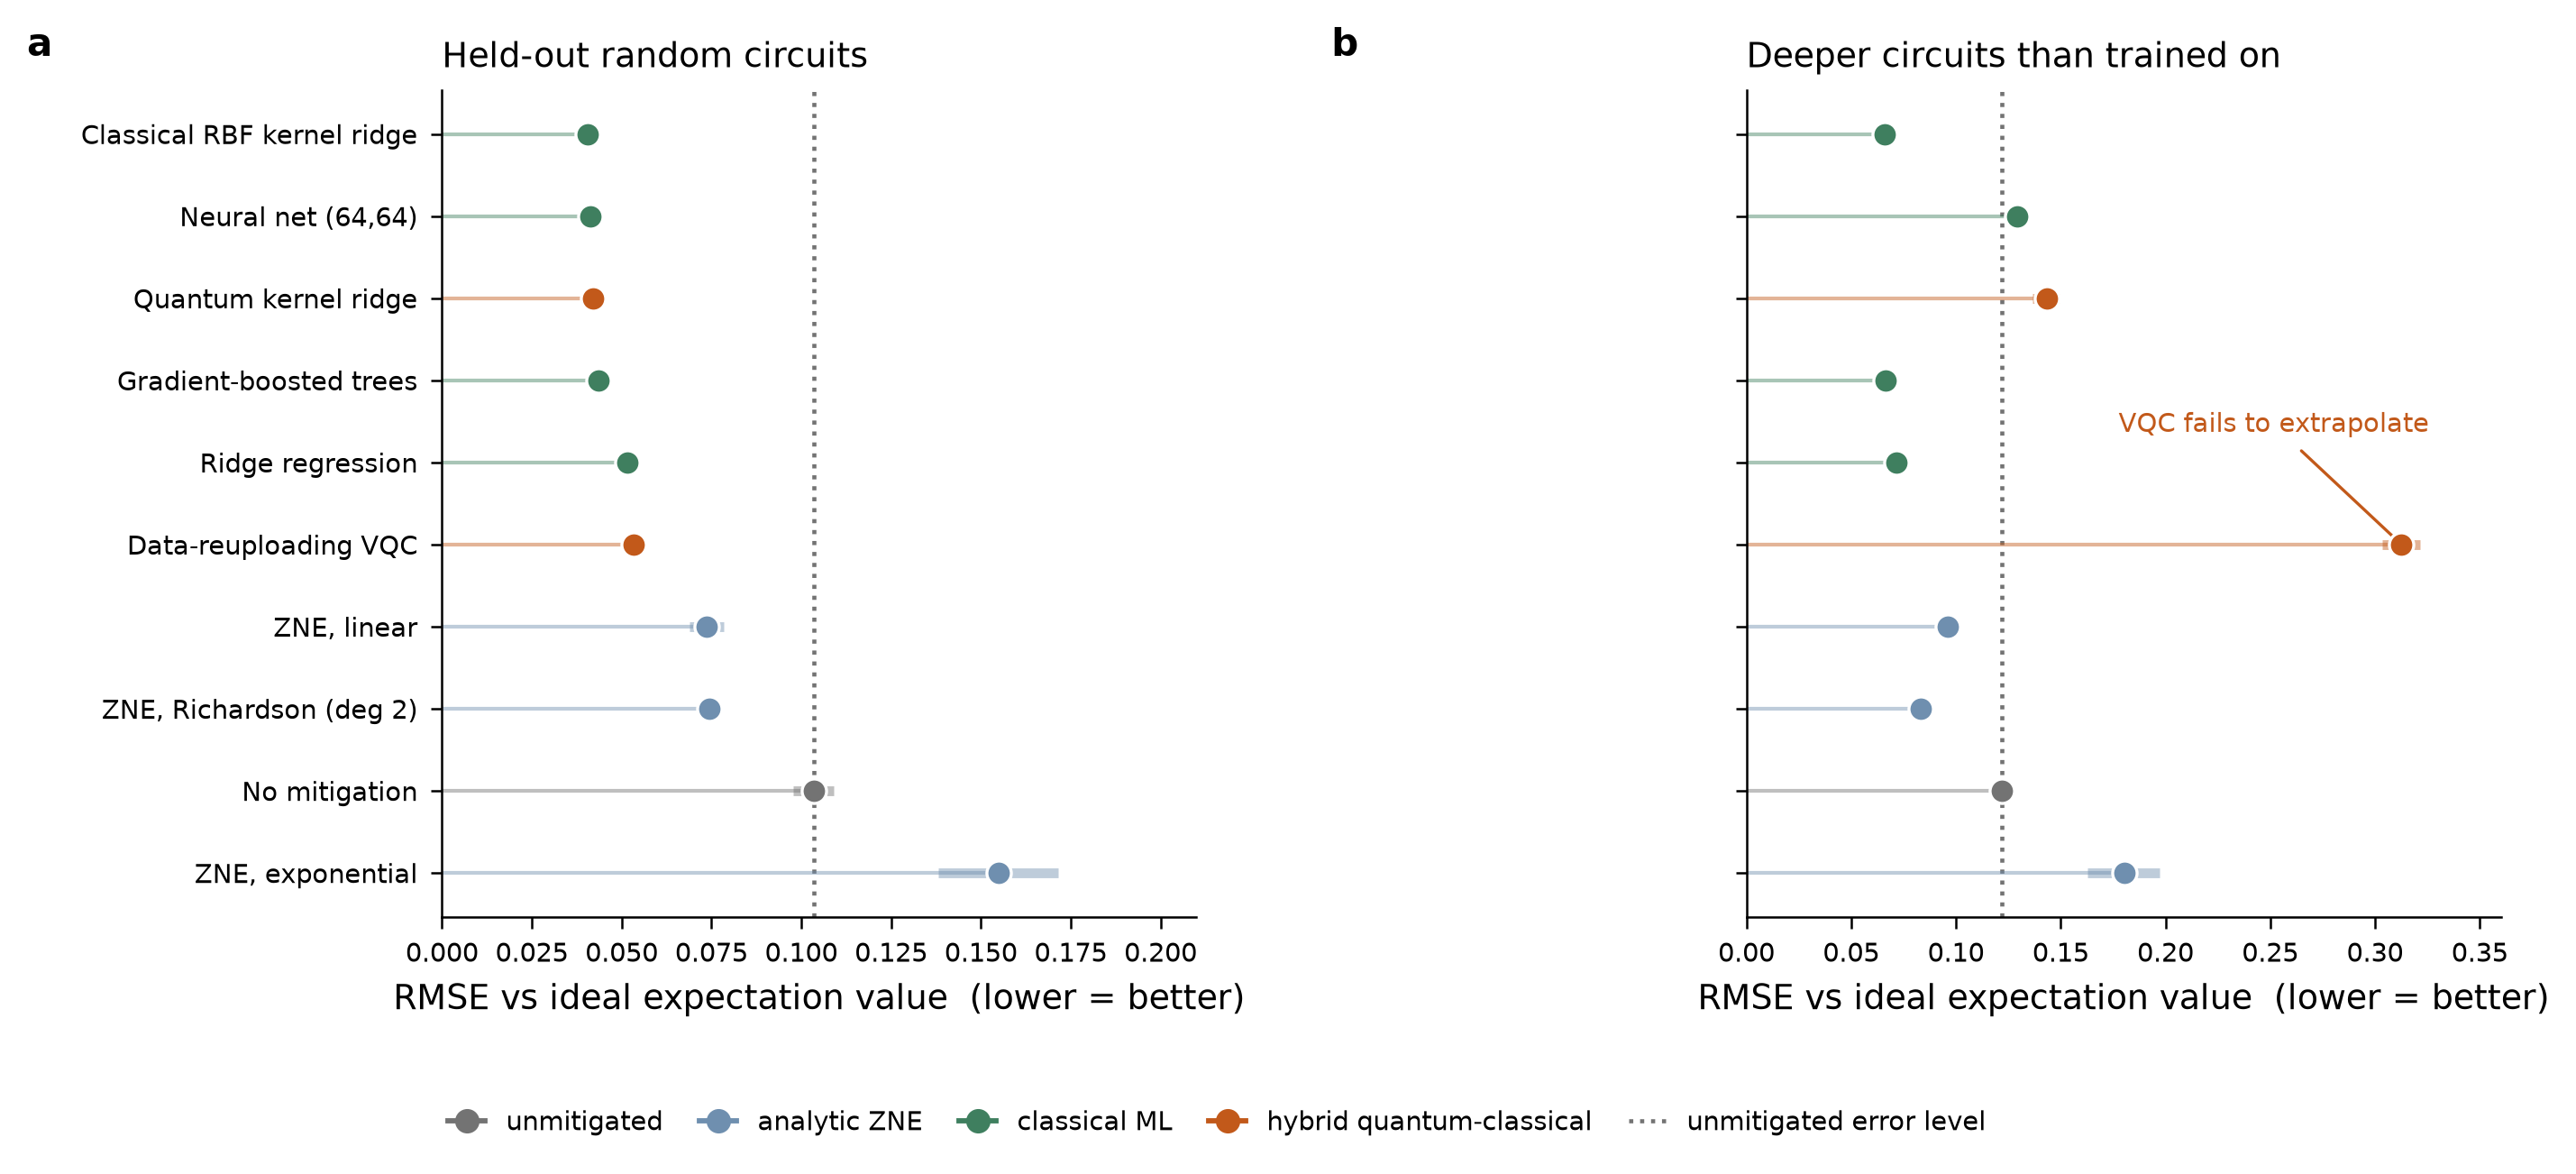
\includegraphics[width=\textwidth]{figures/ch5/fig_ch5_main.png}
\caption[Main benchmark on both splits]{Main benchmark on both splits. Points are RMSE, bars are $95\%$ bootstrap
confidence intervals, and the dotted line marks the unmitigated error level.
Both panels order the arms by Split~A error. Learned methods lead
in-distribution (panel~a); on deeper circuits (panel~b) the neural network, the
quantum kernel and the data-reuploading VQC are worse than the unmitigated baseline.
The VQC point is a single initialisation seed.}
\label{fig:ch5_main}
\end{figure}

\subsection{In-distribution performance on common test circuits}

On Split~A the matched classical RBF and fidelity kernels reach
$0.0404$ and $0.0421$ RMSE, respectively. The neural
network reaches $0.0412$. Linear extrapolation, the strongest
analytic arm on this split, reaches $0.0737$. Relative to linear ZNE, RBF
lowers RMSE by $45.2\%$. The paired difference
RMSE(RBF) $-$ RMSE(fidelity) is $-0.00168$ (95\% CI $[-0.00324,\allowbreak -0.00071]$).
Its interval favours RBF. Section~\ref{sec:ch5_robustness} reports
the comparison over ten additional circuit-grouped holdouts.

Linear ridge regression reaches $0.0515$ and improves on every analytic method
on Split~A. Exponential extrapolation reaches $0.1548$, which is $49.6\%$ above
the unmitigated RMSE. Fitting a three-parameter curve with three noisy observations
leaves no redundant measurements to constrain the extrapolation.
Appendix~\ref{sec:appA_exp} describes the resulting sensitivity to shot noise.

\subsection{Out-of-distribution depth extrapolation}

Split~B trains at depth four or less and tests at depth five or six. Boosted
trees reach $0.0665$, linear ridge reaches
$0.0717$, and Richardson extrapolation reaches
$0.0831$. The unmitigated RMSE is
$0.1217$. The neural network and data-reuploading VQC reach $0.1292$ and $0.3127$.

The classical RBF kernel reaches $0.0658$ and the
fidelity kernel reaches $0.1433$ with identical inputs.
The paired difference is $-0.07751$ (95\% CI $[-0.08270,\allowbreak -0.07226]$). Circuit depth and
two-qubit count are proportional at fixed system size in this dataset.
Their values on the deeper circuits fall outside the training range.
The ablation of Section~\ref{sec:ch5_robustness} measures the effect
of removing these inputs.

\subsection{Where the error concentrates}

Figure~\ref{fig:ch5_breakdown} breaks Split~A error down by circuit depth and by
observable.

\begin{figure}[htbp]
\centering
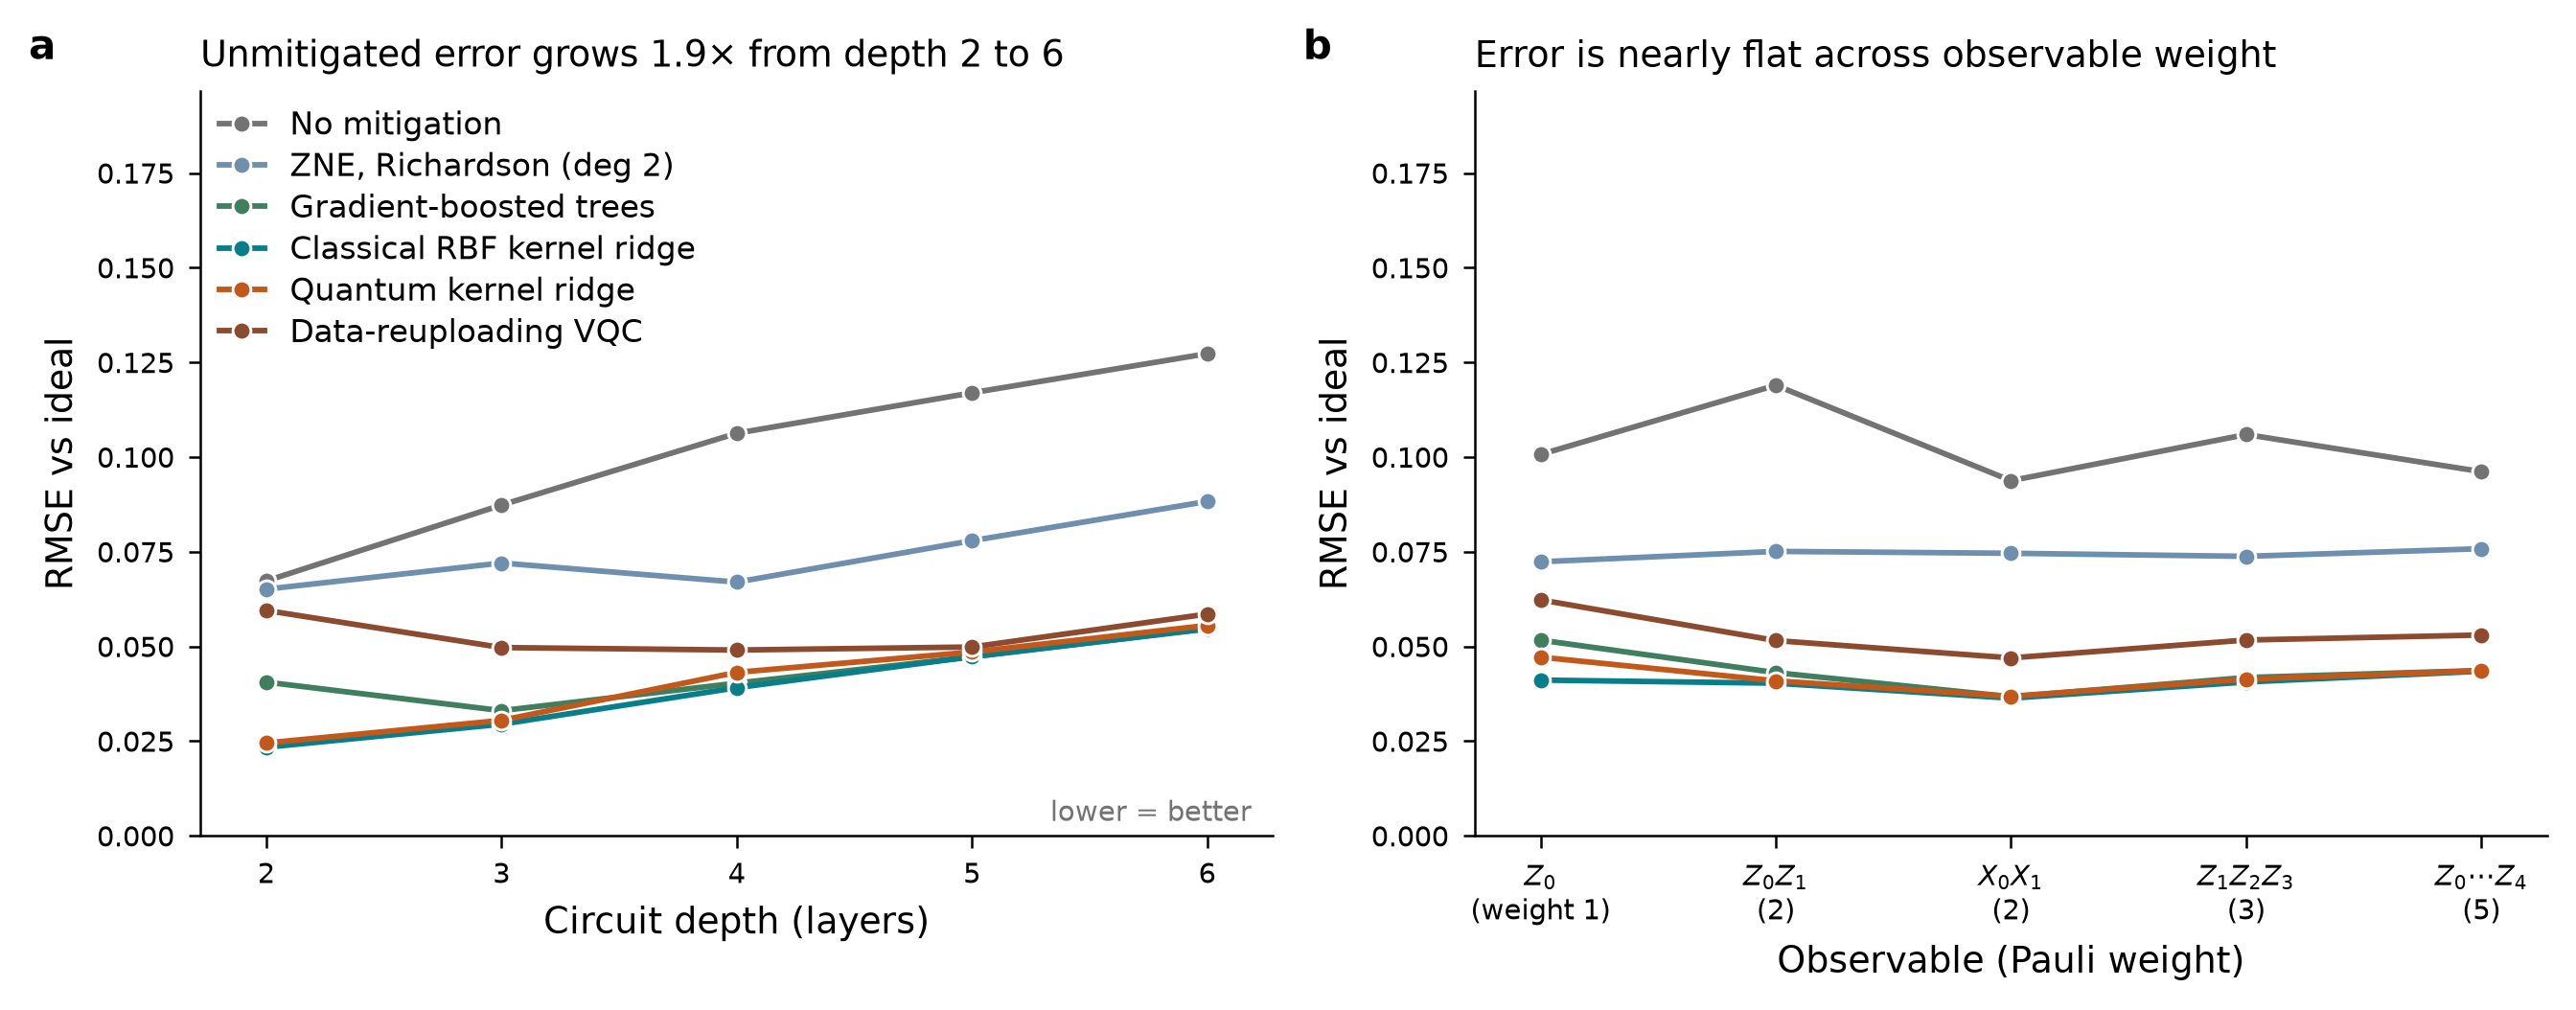
\includegraphics[width=\textwidth]{figures/ch5/fig_ch5_breakdown.png}
\caption[Split~A error by circuit depth and by observable]{Split~A error by circuit depth (panel~a) and by observable (panel~b), for
six representative arms, including both kernels. Unmitigated RMSE grows $1.9\times$
from depth 2 to depth 6 and varies modestly across the five observables.}
\label{fig:ch5_breakdown}
\end{figure}

Unmitigated RMSE rises monotonically from $0.067$ at depth 2 to $0.127$ at depth 6.
Gradient-boosted trees dip from $0.0406$ at depth 2 to $0.0330$ at depth 3 before
rising to $0.0546$ at depth 6, and Richardson extrapolation dips at depth 4.
At each depth and for each observable, the two kernels use the same test circuits.

\section{Fidelity-kernel bandwidth sensitivity}
\label{sec:ch5_bandwidth}

The quantum-kernel arm in Table~\ref{tab:ch5_main} has its bandwidth $\beta$ tuned
by cross-validation. Table~\ref{tab:ch5_bandwidth} and Figure~\ref{fig:ch5_bandwidth}
report performance at fixed bandwidths, with the ridge penalty reselected by
cross-validation at each bandwidth.

\begin{table}[htbp]
\centering
\caption[Quantum-kernel bandwidth sensitivity]{Quantum-kernel bandwidth sensitivity on Split~A. The mean off-diagonal
Gram matrix entry measures how similar the embedded states are on average: a value
near one means most pairs are nearly identical, a value near zero means most are
nearly orthogonal. Unmitigated RMSE on this fold is $0.1035$.}
\label{tab:ch5_bandwidth}
\small
\begin{tabular}{ccccc}
\toprule
\textbf{Bandwidth $\beta$} & \textbf{RMSE (95\% CI)} & \textbf{Red.\ \%}
& \textbf{Mean off-diag.\ $k$} & \textbf{CV $R^2$} \\
\midrule
0.02 & 0.0433 (0.0408--0.0458) & 58.1 & 0.9988 & 0.963 \\
0.05 & 0.0422 (0.0396--0.0444) & 59.2 & 0.9924 & 0.966 \\
0.15 & 0.0421 (0.0394--0.0449) & 59.3 & 0.9339 & 0.967 \\
0.40 & 0.0481 (0.0422--0.0552) & 53.5 & 0.6737 & 0.941 \\
1.00 & 0.1526 (0.1366--0.1695) & $-47.4$ & 0.2041 & 0.577 \\
2.00 & 0.2371 (0.2210--0.2532) & $-129.1$ & 0.0558 & 0.124 \\
\bottomrule
\end{tabular}
\end{table}

\begin{figure}[htbp]
\centering
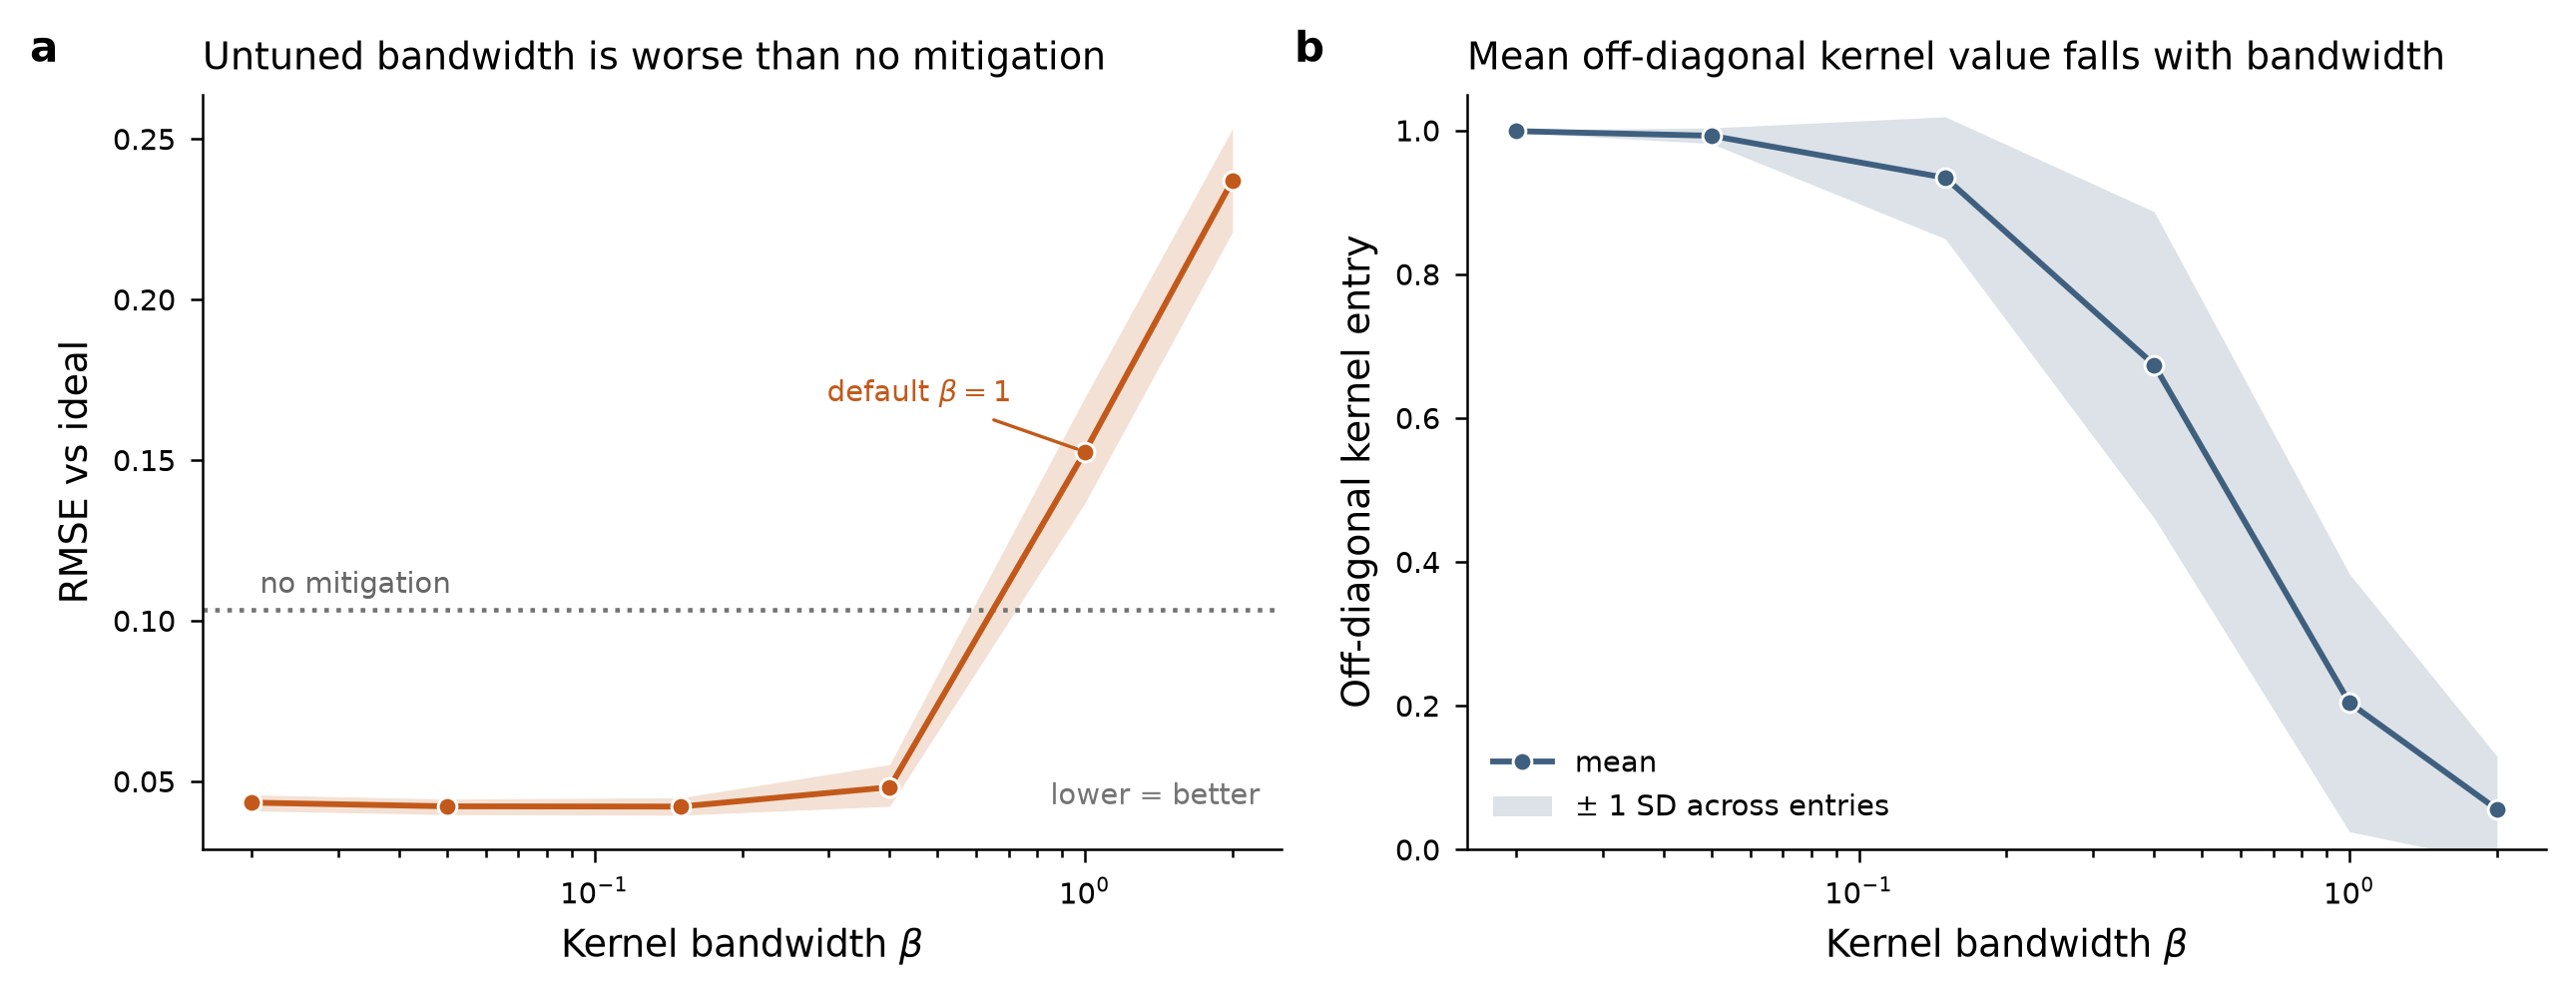
\includegraphics[width=0.95\textwidth]{figures/ch5/fig_ch5_bandwidth.png}
\caption[Bandwidth sensitivity of fidelity-kernel ridge regression]{Bandwidth sensitivity of fidelity-kernel ridge regression on Split~A.
Panel~a: RMSE against bandwidth, with the shaded band the $95\%$ bootstrap interval
and the dotted line the unmitigated error level. Panel~b: the mean off-diagonal
entry of the Gram matrix over the same bandwidths; the band is $\pm 1$ standard
deviation across entries.}
\label{fig:ch5_bandwidth}
\end{figure}

The fixed-bandwidth fidelity study gives RMSE $0.1526$ at
$\beta=1$ and a minimum observed error of $0.0421$ at
$\beta=0.15$. The off-diagonal kernel entries change as
bandwidth spreads the embedded data. The resulting error spread motivates
a tuned bandwidth for each fidelity comparison.

\section{Noise-strength sweep}\label{sec:ch5_noise}

Experiment E1 multiplies the base rates $(p_1,p_2,\gamma)$ by
$m\in\{0.5,1,2,4\}$ while retaining the three extrapolation scales
$\lambda\in\{1,2,3\}$. At $m=4$ and $\lambda=1$, the depolarising channel
following a two-qubit gate has probability $m p_2=0.08$ on each wire,
independently. The probability of a nonidentity Pauli on at least one wire at
that scale is $1-(1-0.08)^2=0.1536$.

Every multiplier uses the same $500$ five-qubit circuits, ideal
targets, and seed-7 circuit-grouped split of $350$ training and $150$ held-out
circuits. Circuit angles are drawn once. A separate random stream for each
multiplier samples $4096$ shots per expectation value. The models use
the same reduced tuning budget at all four multipliers, including
$24$ candidates and four grouped inner folds for each kernel and
$30$ epochs for each variational arm. The $1\times$ dataset is generated
on this shared E1 pool.

\begin{figure}[htbp]
\centering
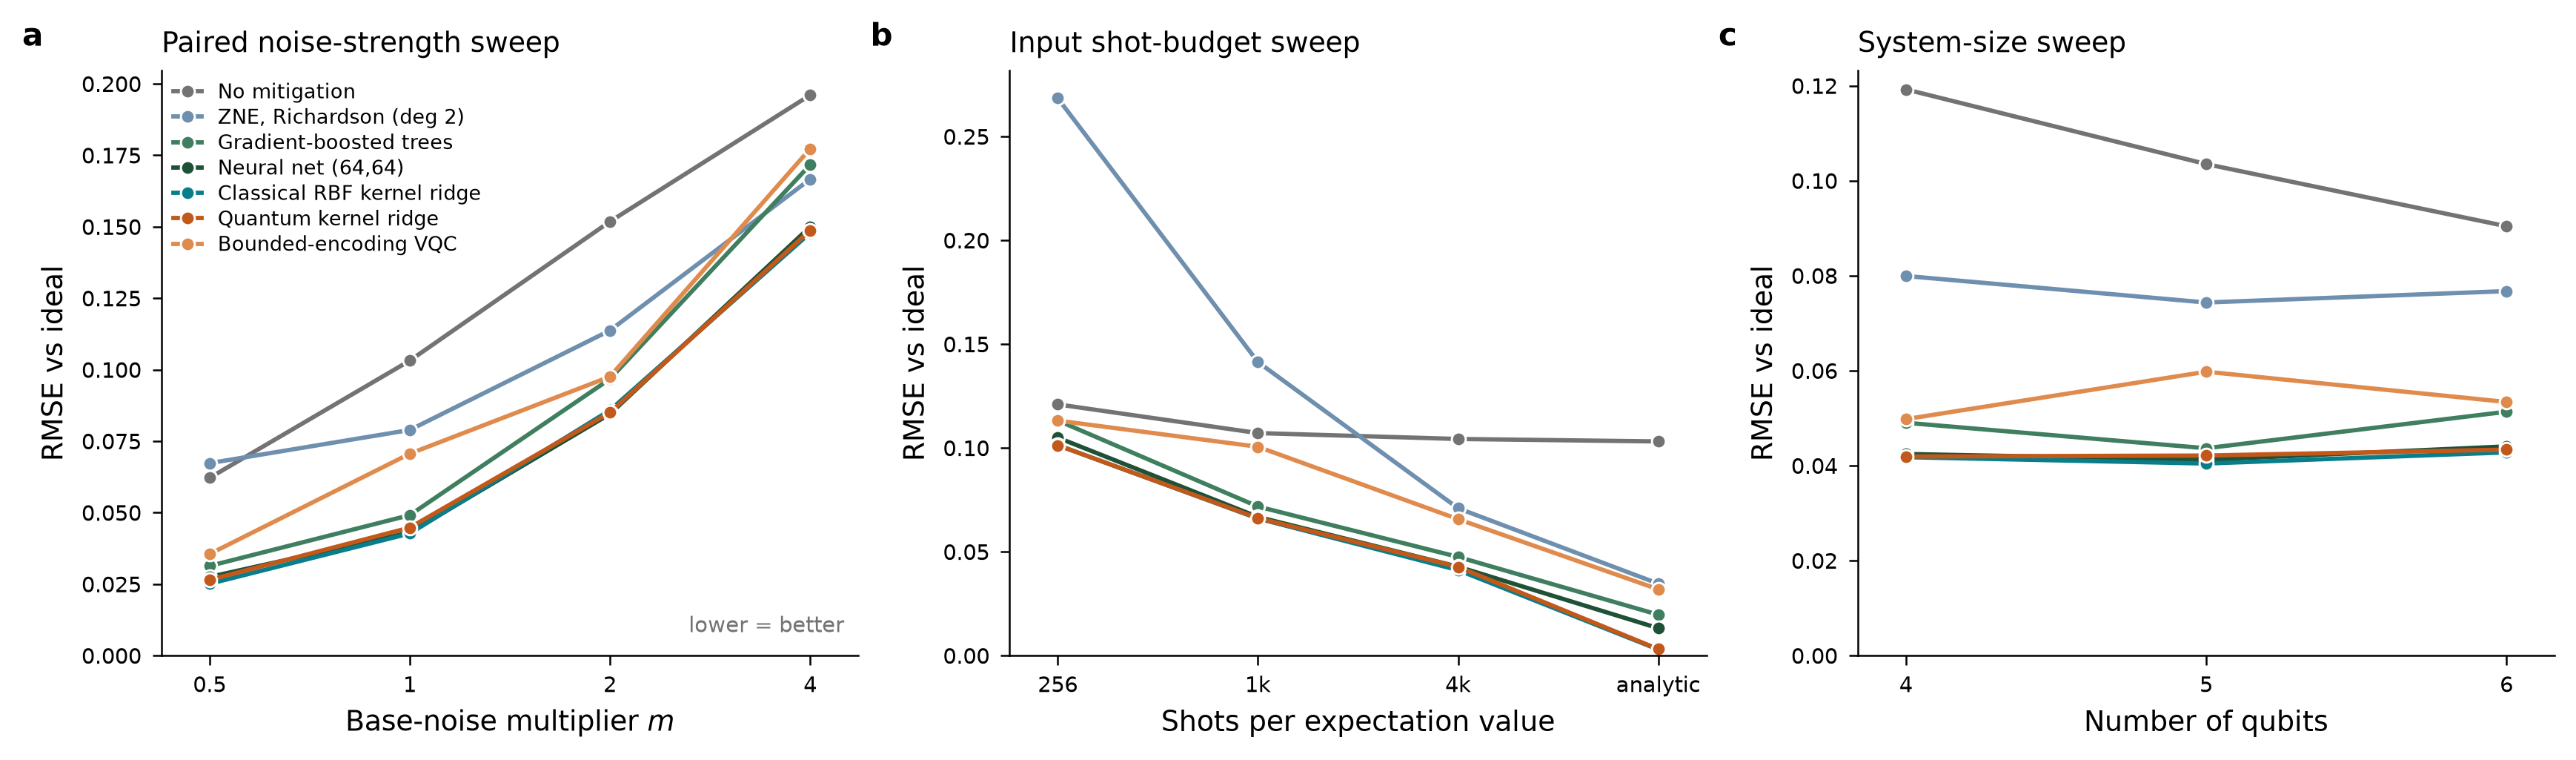
\includegraphics[width=\textwidth]{figures/ch5/fig_ch5_sweeps.png}
\caption[Sweeps over noise strength, shot budget and qubit count]{Sweeps on held-out random circuits. Panel~a varies the base-noise multiplier
with the same circuit pool, grouped split and tuning budget. Panel~b varies the
shots per expectation value, with ``analytic'' denoting the limit without
sampling noise. Panel~c varies qubit count. Every panel plots RMSE against the
ideal expectation value. The grey series is the unmitigated baseline.}
\label{fig:ch5_sweeps}
\end{figure}

Unmitigated RMSE rises from $0.0621$ at $0.5\times$ to $0.1960$ at $4\times$.
Absolute RMSE rises at each step for ten of the eleven methods, with
exponential extrapolation the exception. The classical RBF kernel reduces
unmitigated RMSE by $59.6\%$, $58.6\%$, $43.5\%$ and $24.6\%$ as $m$ increases.
It gives the lowest observed RMSE at $0.5\times$, $1\times$ and $4\times$,
and the neural network gives the lowest at $2\times$. The paired
circuit-bootstrap intervals favour RBF over fidelity at $0.5\times$,
$1\times$ and $4\times$ and include zero at $2\times$.

\section{Observable shot-budget sweep}\label{sec:ch5_shots}

Figure~\ref{fig:ch5_sweeps}(b) varies the shots used to estimate each input
observable, from $256$ to exact expectation values. The sweep resamples the
stored exact values using Eq.~\eqref{eq:ch3_shots} and refits on the same
circuit-grouped split. Fidelity-kernel entries remain exact throughout.

At $256$ shots, Richardson extrapolation reaches
$0.2684$, consistent with
the variance amplification in Eq.~\eqref{eq:appA_variance}. Across
$256$ shots, $4096$ shots and exact inputs, RBF achieves
$0.1013$, $0.0411$, $0.0029$.
The fidelity-kernel estimates under those same three conditions are
$0.1013$, $0.0427$, $0.0031$.

\section{System-size sweep}\label{sec:ch5_qubits}

Figure~\ref{fig:ch5_sweeps}(c) compares $4$, $5$ and $6$ qubits.
The classical RBF RMSEs are
$0.0418$, $0.0404$, $0.0428$,
and the corresponding fidelity-kernel RMSEs are
$0.0419$, $0.0421$, $0.0434$.
The settings differ in their circuit and observable construction and span
a small size range. The comparison describes the three tested settings.

\section{Learning curves}\label{sec:ch5_learning}

A practitioner's real constraint is how many reference circuits must be simulated to
train a mitigation model. Figure~\ref{fig:ch5_learning} varies the training set from
$31$ to $630$ circuits.

\begin{figure}[htbp]
\centering
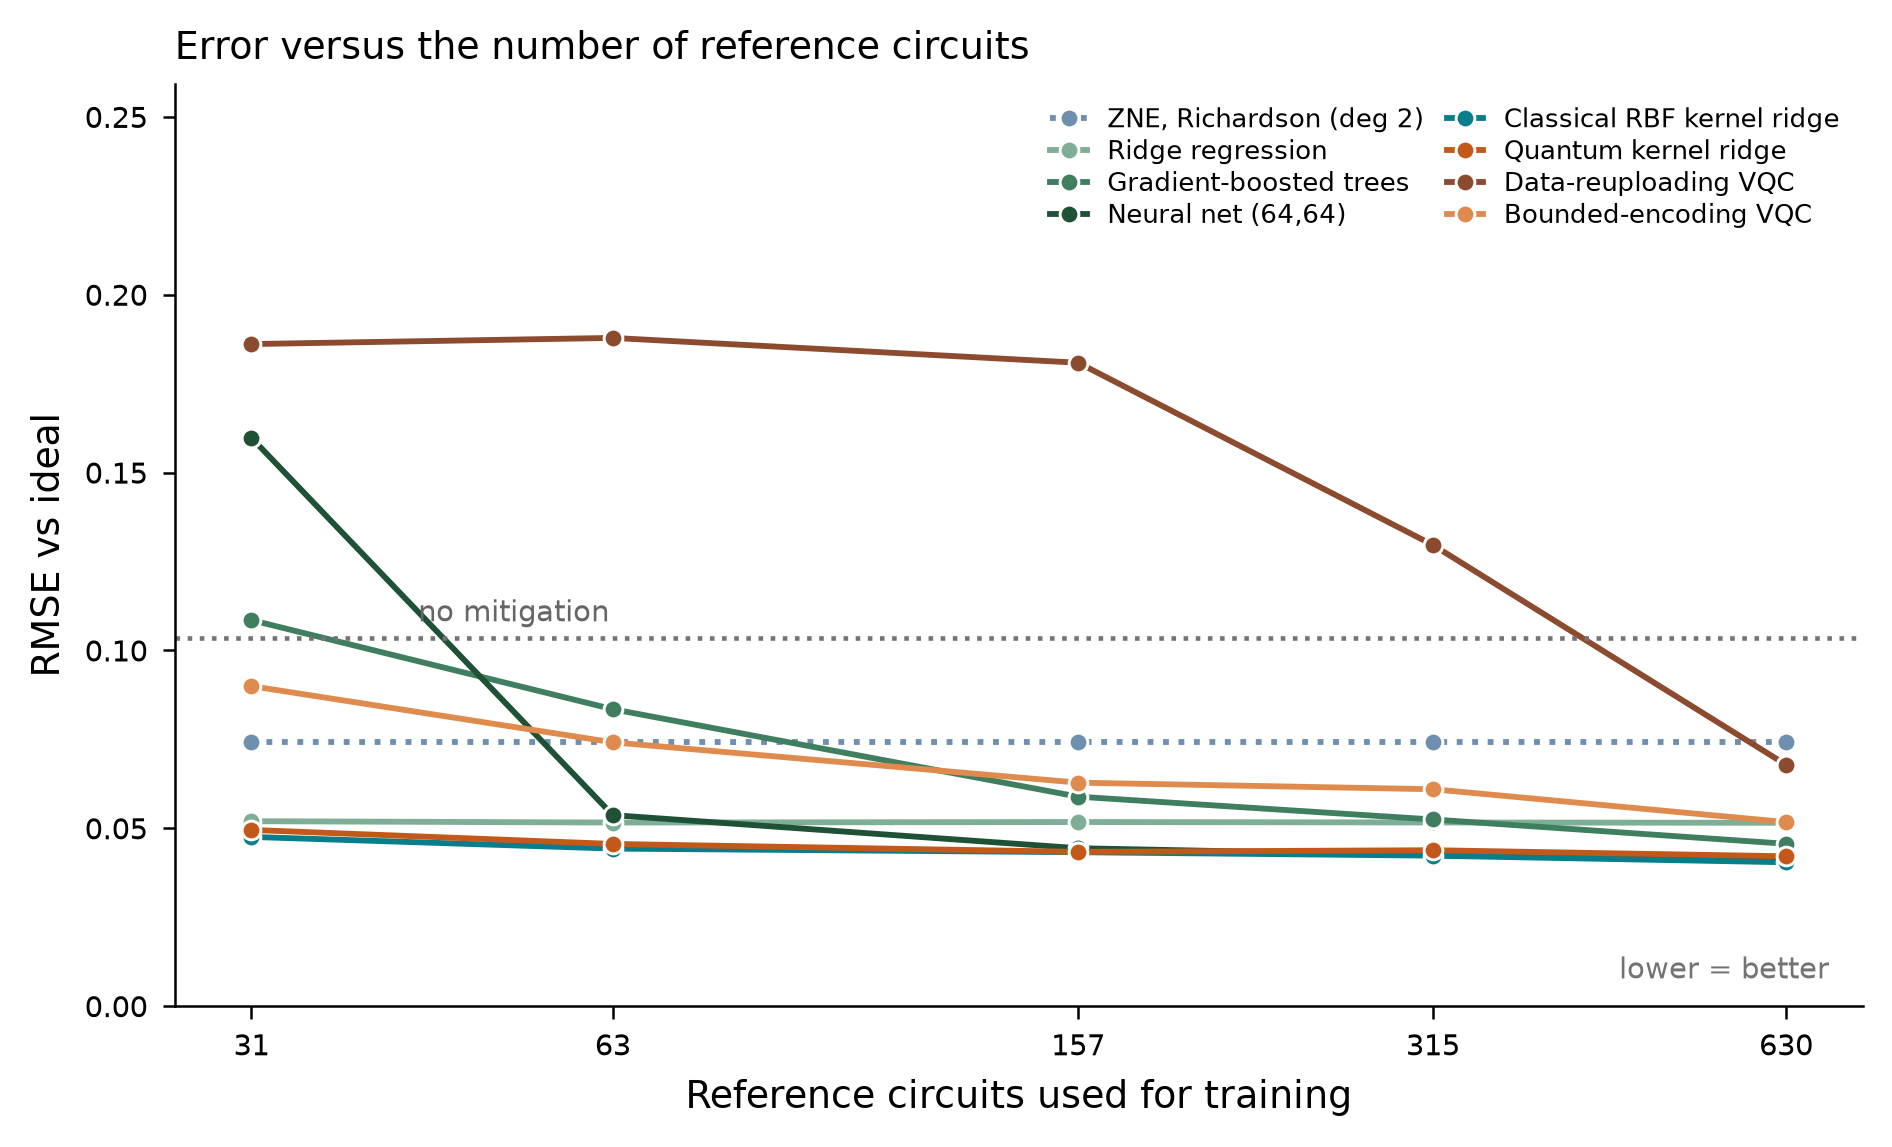
\includegraphics[width=0.8\textwidth]{figures/ch5/fig_ch5_learning.png}
\caption[Learning curves on held-out random circuits]{Learning curves on held-out random circuits, one random subset of
reference circuits per training size. The analytic Richardson arm is drawn as a flat
dotted line because it requires no training. Section~\ref{sec:ch5_learning} reports
the spread over $20$ subsets at the two smallest sizes.}
\label{fig:ch5_learning}
\end{figure}

Each point of Figure~\ref{fig:ch5_learning} is one random subset of training
circuits, so the curve alone cannot separate sample efficiency from the luck of a
draw. At the two smallest sizes the experiment was therefore repeated over $20$
independent subsets (the variational arms are excluded because of their training cost).

At $31$ training circuits, the RBF and fidelity kernels reach
$0.0623\pm0.0220$ and
$0.0582\pm0.0143$ across the
$20$ draws. At $63$ circuits, their mean RMSEs are
$0.0489$ and $0.0499$.
The spread comes from changing reference circuits while holding the test set fixed.
At $31$ circuits, the paired intervals favour RBF in
$4$
draws and fidelity in
$9$.

\section{Feature ablation}\label{sec:ch5_ablation}

Table~\ref{tab:ch5_ablation} removes information from the feature vector to see where
the learned advantage comes from.

\begin{table}[htbp]
\centering
\caption[Feature ablation on Split~A]{Feature ablation on Split~A (RMSE). ``Noise-scaled only'' uses the three
noise-scaled expectation values, the same information an analytic extrapolation
consumes; ``native + structure'' uses the native noisy value plus the three structural descriptors; ``full'' uses all six features. Unmitigated RMSE is $0.1035$.
The bounded VQC uses the 30-epoch sweep budget.}
\label{tab:ch5_ablation}
\small
\begin{tabular}{lccc}
\toprule
\textbf{Method} & \textbf{Noise only} & \textbf{Native + structure}
& \textbf{Full} \\
\midrule
Ridge regression & 0.0515 & 0.0725 & 0.0515 \\
Gradient-boosted trees & 0.0528 & 0.0482 & 0.0456 \\
Neural net (64,64) & 0.0474 & 0.0444 & 0.0412 \\
Classical RBF kernel ridge & 0.0476 & 0.0440 & 0.0404 \\
Quantum kernel ridge & 0.0497 & 0.0457 & 0.0421 \\
Bounded-encoding VQC & 0.0553 & 0.0653 & 0.0517 \\
\bottomrule
\end{tabular}
\end{table}

On the three noise-scale inputs alone, RBF and fidelity reach
$0.0476$ and
$0.0497$. Linear extrapolation
reaches $0.0737$ on the same test fold. With the native noisy measurement
and the three structural descriptors, the kernels reach
$0.0440$ and
$0.0457$.
Both kernels use the reduced grid in each feature condition.

\section{Bounded encoding under depth extrapolation}
\label{sec:ch5_bounded}

Table~\ref{tab:ch5_bounded} adds the bounded-encoding arm to the depth-extrapolation
comparison. On Split~B, data reuploading gives $2.57$ times the unmitigated RMSE.
The periodic encoding $R_Y(w \cdot x + b)$ can map distinct feature values to
equivalent rotations. The bounded variant of Eq.~\eqref{eq:ch3_bounded} uses
a $\tanh$ transform to confine angles to $[-\pi/2, \pi/2]$. The transform also
changes angles within the training range, so this is a comparison of the two
encodings as fitted.

\begin{table}[htbp]
\centering
\caption[Depth extrapolation with the bounded-encoding arm]{Depth-extrapolation experiment with the bounded-encoding arm added
(Split~B: train depth $\leq 4$, test depth $\geq 5$). Unmitigated RMSE is $0.1217$.}
\label{tab:ch5_bounded}
\small
\begin{tabular}{lccc}
\toprule
\textbf{Method} & \textbf{RMSE (95\% CI)} & \textbf{Red.\ \%} & \textbf{Verdict} \\
\midrule
Classical RBF kernel ridge & 0.0658 (0.0629--0.0685) & 46.0 & lowest RMSE \\
Gradient-boosted trees & 0.0665 (0.0637--0.0691) & 45.4 & lower error \\
Ridge regression & 0.0717 (0.0685--0.0741) & 41.1 & lower error \\
ZNE, Richardson (deg 2) & 0.0831 (0.0803--0.0854) & 31.8 & lower error \\
ZNE, linear & 0.0960 (0.0921--0.0996) & 21.2 & lower error \\
No mitigation & 0.1217 (0.1174--0.1258) & 0.0 & reference \\
Neural net (64,64) & 0.1292 (0.1251--0.1339) & $-6.2$ & higher error \\
Quantum kernel ridge & 0.1433 (0.1369--0.1493) & $-17.7$ & higher error \\
Bounded-encoding VQC & 0.1543 (0.1486--0.1591) & $-26.7$ & higher error \\
ZNE, exponential & 0.1805 (0.1628--0.1962) & $-48.3$ & higher error \\
Data-reuploading VQC & 0.3127 (0.3028--0.3215) & $-156.8$ & higher error \\
\bottomrule
\end{tabular}
\end{table}

\begin{figure}[htbp]
\centering
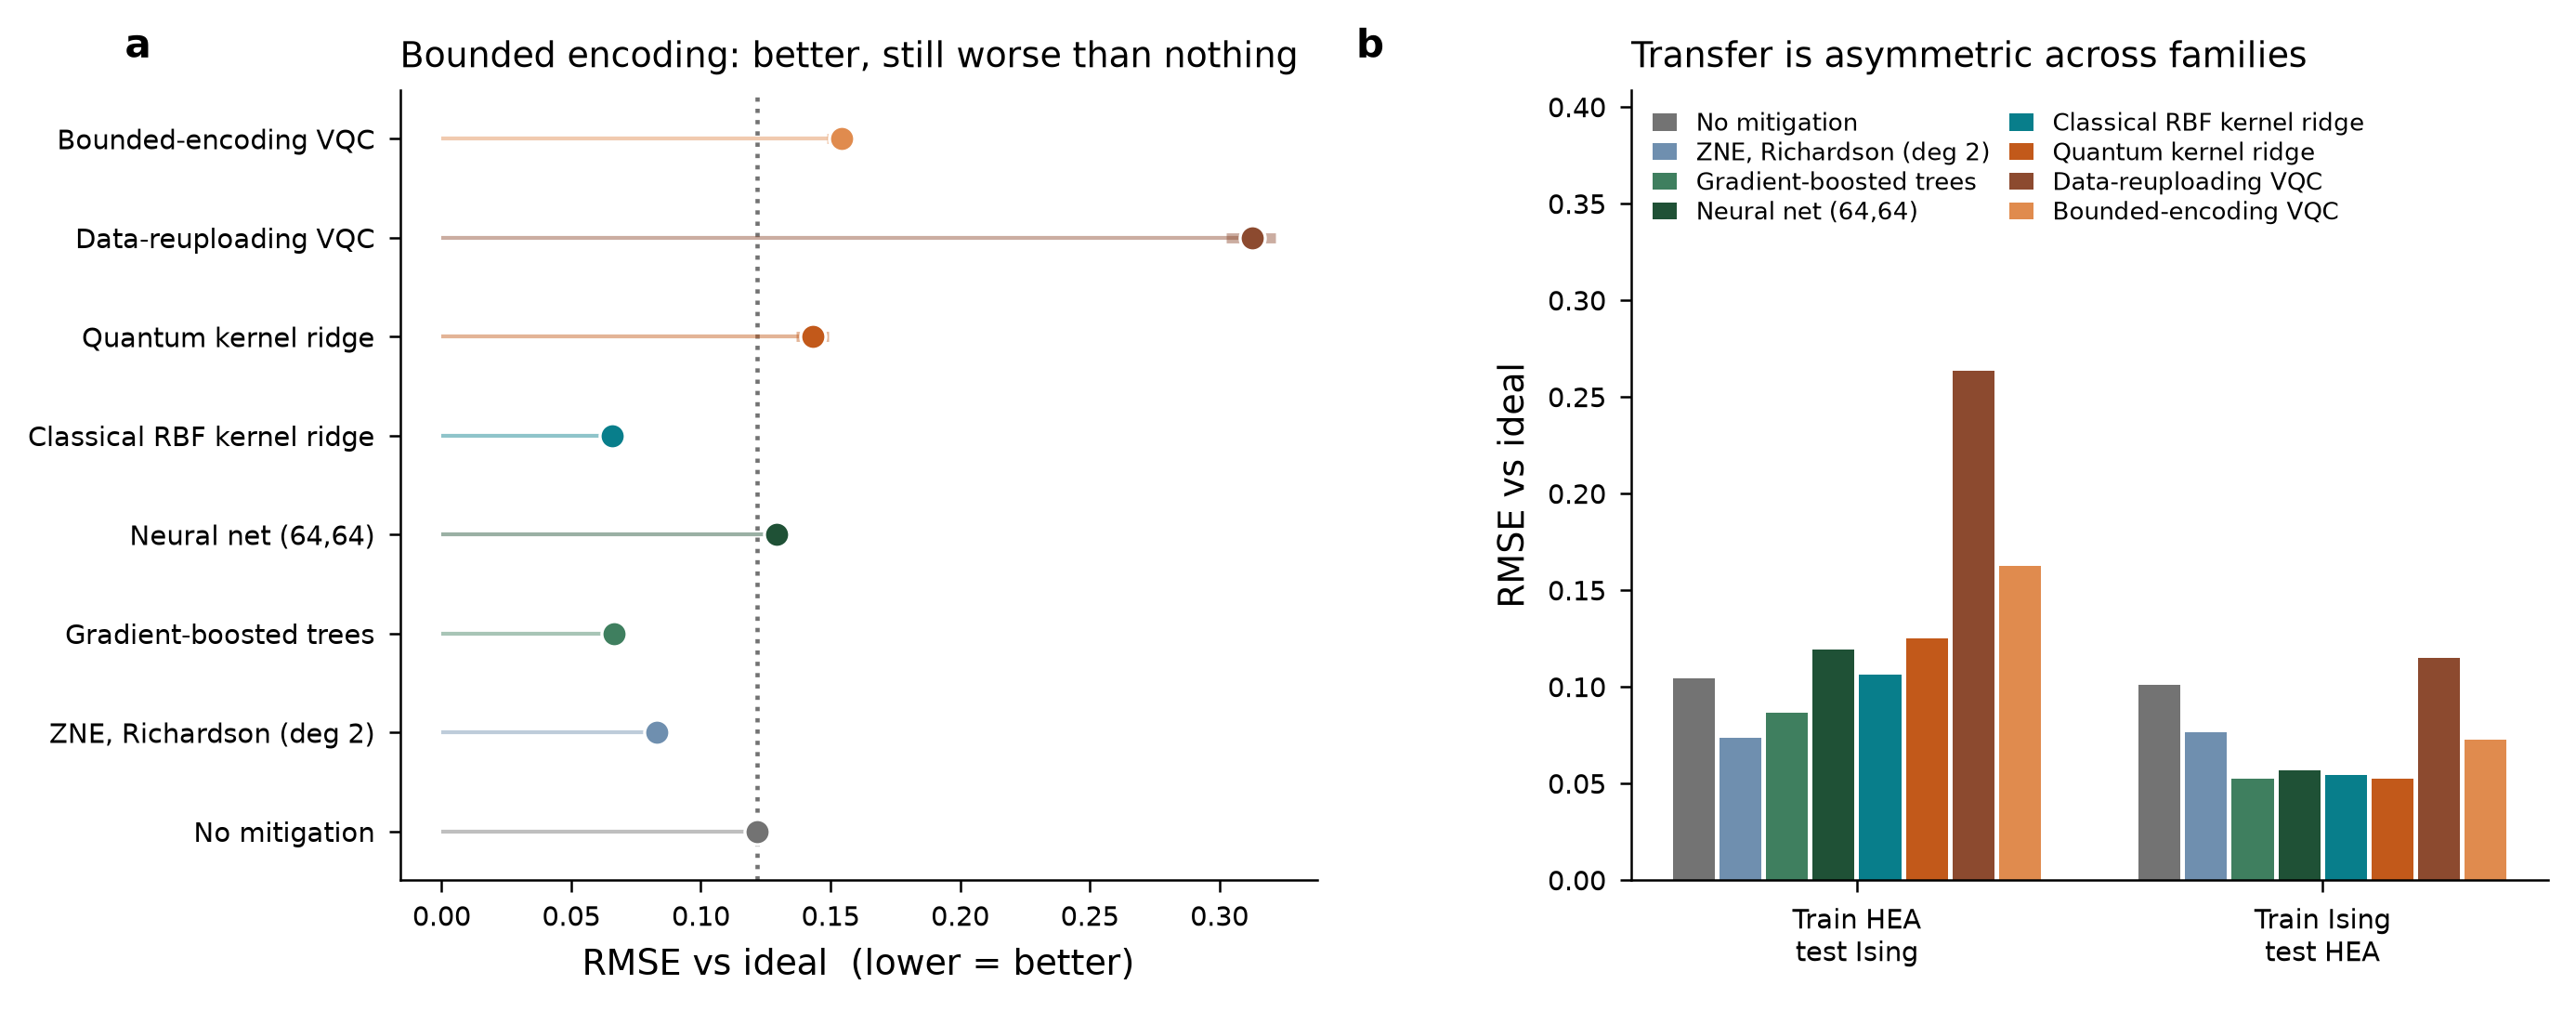
\includegraphics[width=\textwidth]{figures/ch5/fig_ch5_ood.png}
\caption[Out-of-distribution behaviour]{Out-of-distribution behaviour. Panel~a: depth extrapolation with the
bounded-encoding arm added; the dotted line is the unmitigated error level.
Panel~b: cross-family transfer in both directions.}
\label{fig:ch5_ood}
\end{figure}

The bounded VQC reduces full-input RMSE from $0.3127$ to $0.1543$ on the depth
split. Both errors exceed the unmitigated RMSE of $0.1217$. The feature ablation
in Section~\ref{sec:ch5_robustness} compares the two encodings after input
removal and refitting.

\section{Cross-family transfer}\label{sec:ch5_transfer}

Figure~\ref{fig:ch5_ood}(b) trains on one circuit family and tests on the other.
The result is strikingly asymmetric.

With Ising-family training and hardware-efficient testing, RBF and fidelity
reduce error by $46.3\%$
and $48.2\%$.
In the reverse direction, their reductions are
$-2.0\%$ and
$-19.8\%$.
The Ising-to-HEA RBF-minus-fidelity difference is
$+0.00192$ (95\% CI $[+0.00138,\allowbreak +0.00247]$).
Linear extrapolation improves on the raw measurements in both directions.

The ideal target values have different spreads across the two circuit
families. The Ising-family SD is $0.286$, and the hardware-efficient
family SD is $0.189$. The transfer experiment changes the entire circuit
family. Target support is one plausible source of the observed asymmetry.

\section{Cost accounting}\label{sec:ch5_cost}

Table~\ref{tab:ch5_cost} reports circuit settings per prediction and the
observed simulator fit times. The shot-resolved kernel analysis in
Section~\ref{sec:ch5_shotkernel} counts the repetitions of these settings.

\begin{table}[htbp]
\centering
\caption[Cost per method]{Circuit settings per prediction before shots.
Kernel ridge has one dual coefficient per training row. Training times are
wall times from this run, with other configurations executing concurrently
in the environment in Table~\ref{tab:ch4_stack}. Three noise-scaled inputs
at $4096$ shots each require $12{,}288$ circuit executions per prediction.}
\label{tab:ch5_cost}
\small
\begin{tabular}{lcccc}
\toprule
\textbf{Method} & \textbf{Settings/estimate} & \textbf{Parameters}
& \textbf{Fit (s)}$^{\circ}$ & \textbf{Split A RMSE} \\
\midrule
No mitigation & 1 & 0 & 0.0 & 0.1035 \\
ZNE, linear & 3 & 0 & 0.0 & 0.0737 \\
ZNE, Richardson (deg 2) & 3 & 0 & 0.0 & 0.0743 \\
ZNE, exponential & 3 & 0 & 0.0 & 0.1548 \\
Ridge regression & 3 & 7 & 0.0 & 0.0515 \\
Gradient-boosted trees & 3 & 4500$^{\dagger}$ & 6.5 & 0.0436 \\
Neural net (64,64) & 3 & 4673 & 0.4 & 0.0412 \\
Classical RBF kernel ridge & 3 & 3150$^{\ddagger}$ & 42.1 & 0.0404 \\
Quantum kernel ridge & \textbf{3 + 3150}$^{\S}$ & 3150$^{\ddagger}$ & 73.0 & 0.0421 \\
Data-reuploading VQC & \textbf{3 + 1} & 114 & 47.4 & 0.0533$^{\P}$ \\
\bottomrule
\end{tabular}
\par\smallskip
\parbox{0.97\linewidth}{\footnotesize
$^{\dagger}$ Total selected tree leaves. $^{\ddagger}$ Dual coefficients.
$^{\S}$ One fidelity setting per training row for overlap measurement.
$^{\P}$ Seed~7 in this fit.
$^{\circ}$ Fits include each arm's tuning procedure.}
\end{table}

On the full feature set, each classical regressor and linear ZNE uses three
noise-scaled measurements for a new prediction. The learned regressors also
require labelled reference data and classical training. RBF evaluates
test-to-training similarities numerically from those same input measurements.

An implementation using a measured fidelity kernel would add $3150$
inversion-test settings per Split~A prediction, one per training row. Its
dense training Gram matrix uses up to $4{,}962{,}825$ settings, counting the
diagonal, before multiplication by shots. For the $1350$ Split~A test rows the
two matrices add up to $9{,}215{,}325$ settings at one fixed bandwidth.
Section~\ref{sec:ch5_shotkernel} measures finite-shot accuracy under this cost
model. The variational circuit adds one inference setting per prediction.

The two kernels use the same prediction features here. Their paired Split~A
accuracy difference is $-0.00168$ (95\% CI $[-0.00324,\allowbreak -0.00071]$).

\section{Robustness to the split, the seed and the input features}
\label{sec:ch5_robustness}

The reference random holdout uses split seed~7. The repeated holdouts use the
reduced hyperparameter grid and $30$-epoch variational budget of the sweeps.
The separate initialisation and feature-set comparisons use the settings
described below.

\paragraph{Ten grouped holdouts.} Table~\ref{tab:ch5_robust} and
Figure~\ref{fig:ch5_robustness}(a) repeat the main comparison over ten repeated
$70/30$ circuit-grouped splits (seeds $100$--$109$). For every split each arm is
compared with the reference arms by the paired bootstrap of
Section~\ref{sec:ch3_metrics}.

\begin{table}[htbp]
\centering
\caption[Idealised regime, ten circuit-grouped splits]{Idealised regime, ten circuit-grouped splits. RMSE is the mean $\pm$ standard
deviation over splits; ``rank'' is the mean rank within a split (1 = best). The last
three columns count the splits, out of ten, in which the paired difference against
the named reference is resolved in the stated direction.}
\label{tab:ch5_robust}
\small
\setlength{\tabcolsep}{5pt}
\begin{tabular}{lccccc}
\toprule
\textbf{Method} & \textbf{RMSE} & \textbf{Rank} & \textbf{Better than} & \textbf{Better than}
& \textbf{Worse than} \\
 & & & \textbf{no mitigation} & \textbf{linear ZNE} & \textbf{neural net} \\
\midrule
Classical RBF kernel ridge & $0.0416 \pm 0.0011$ & 1.1 & 10 & 10 & 0 \\
Quantum kernel ridge & $0.0426 \pm 0.0012$ & 2.4 & 10 & 10 & 1 \\
Neural net (64,64) & $0.0426 \pm 0.0009$ & 2.5 & 10 & 10 & --- \\
Gradient-boosted trees & $0.0471 \pm 0.0010$ & 4.0 & 10 & 10 & 10 \\
Ridge regression & $0.0531 \pm 0.0014$ & 5.3 & 10 & 10 & 10 \\
Bounded-encoding VQC & $0.0552 \pm 0.0032$ & 5.9 & 10 & 10 & 10 \\
ZNE, linear & $0.0738 \pm 0.0018$ & 7.8 & 10 & --- & 10 \\
ZNE, Richardson (deg 2) & $0.0754 \pm 0.0012$ & 8.4 & 10 & 0 & 10 \\
Data-reuploading VQC & $0.0842 \pm 0.0371$ & 7.8 & 8 & 4 & 10 \\
No mitigation & $0.1018 \pm 0.0022$ & 9.8 & --- & 0 & 10 \\
ZNE, exponential & $0.1599 \pm 0.0086$ & 11.0 & 0 & 0 & 10 \\
\bottomrule
\end{tabular}
\end{table}

\begin{figure}[htbp]
\centering
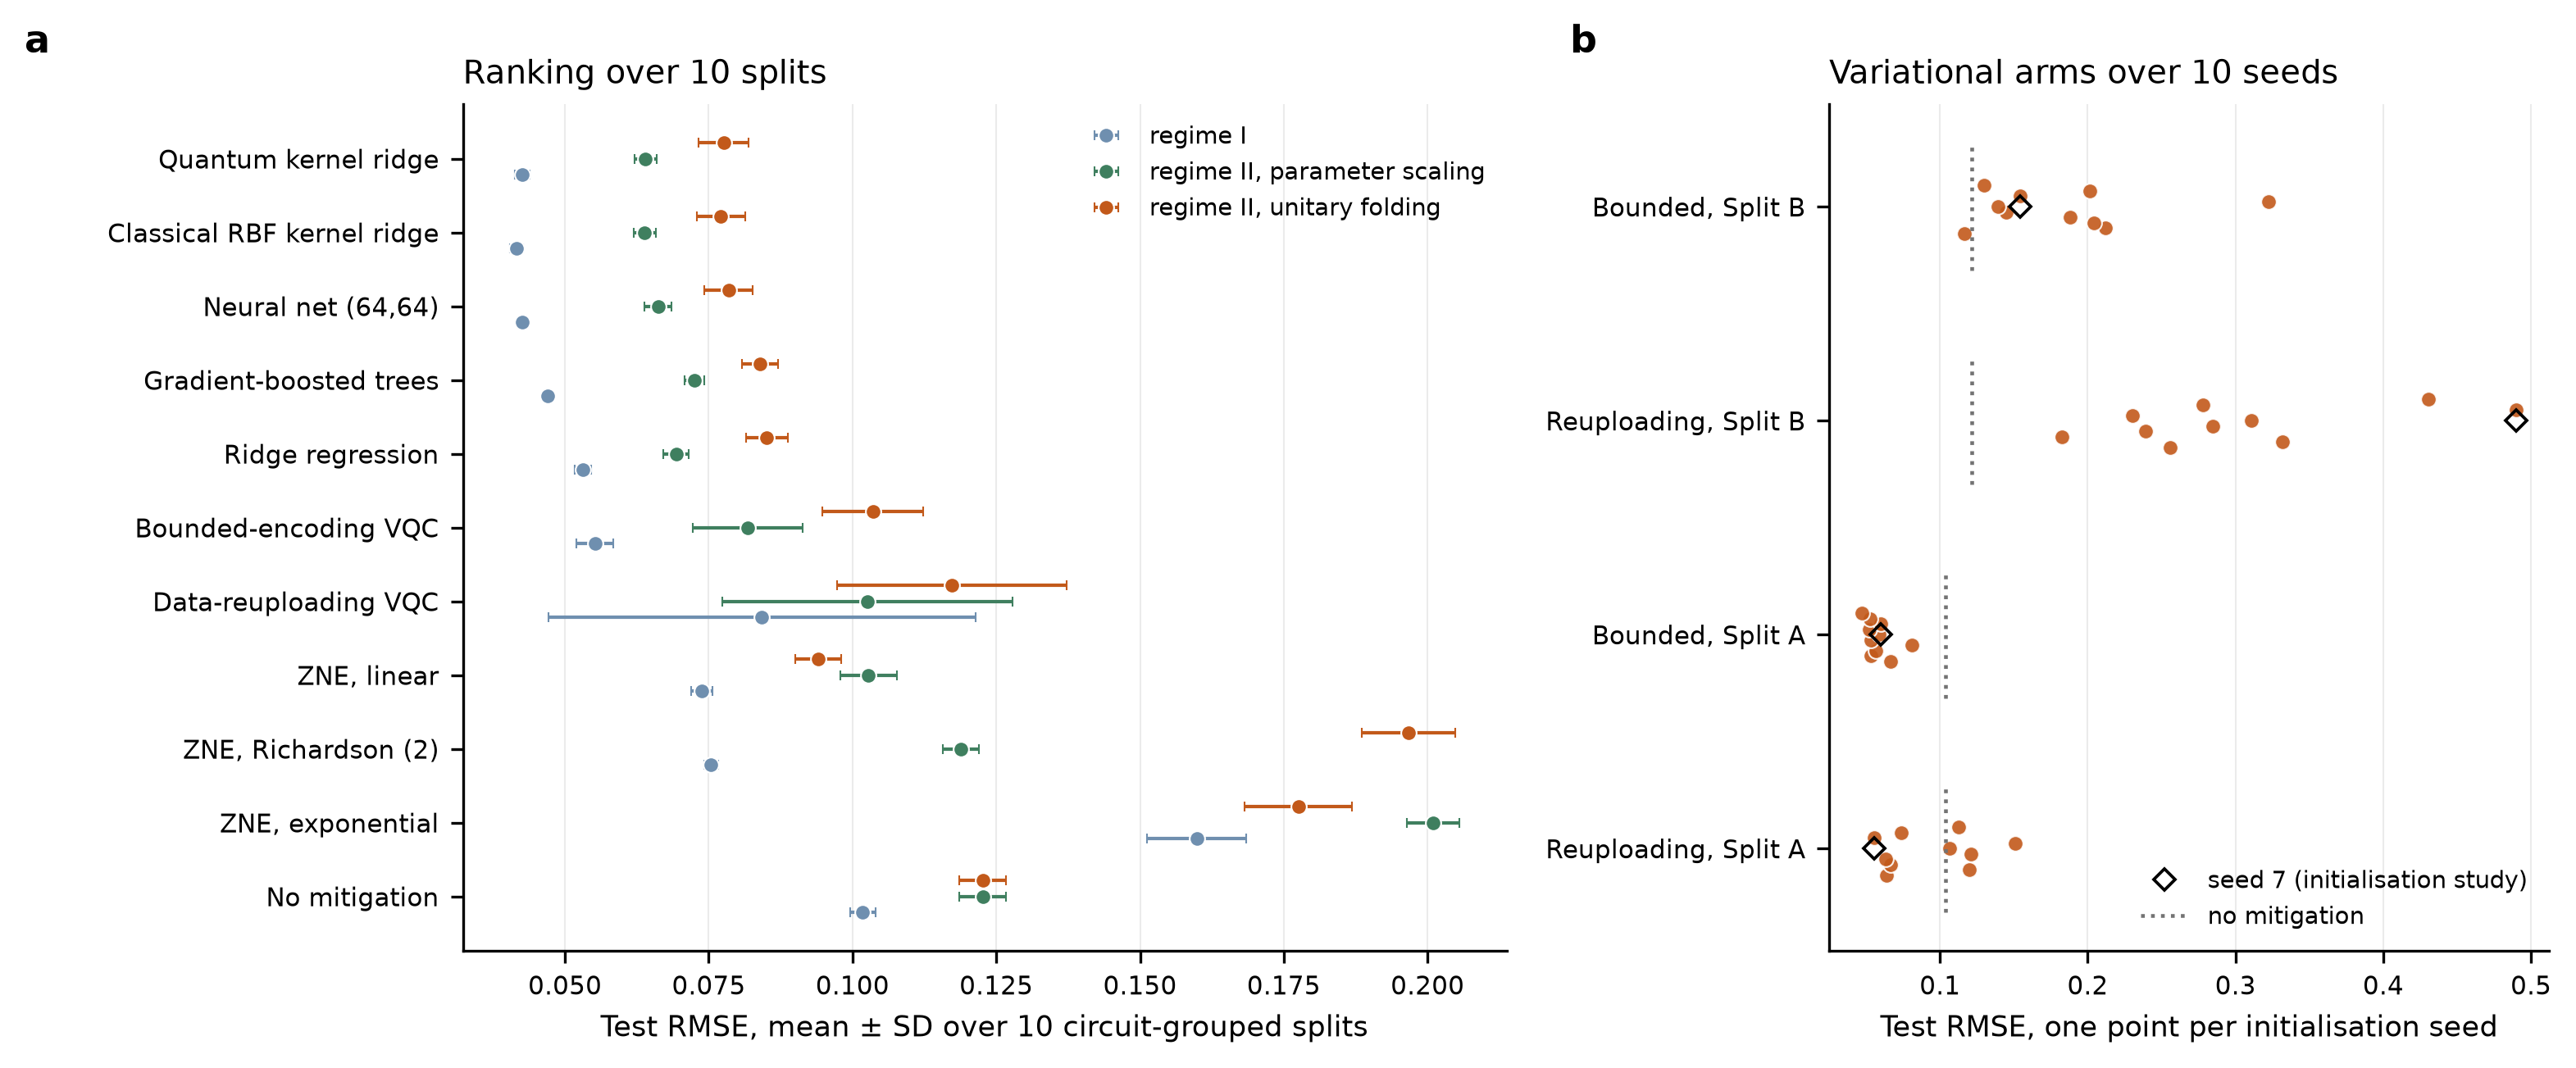
\includegraphics[width=\textwidth]{figures/ch5/fig_ch5_robustness.png}
\caption[Robustness of the ranking over splits and seeds]{Robustness of the ranking. Panel~a: mean $\pm$ one standard deviation of test
RMSE over ten circuit-grouped splits, in the idealised regime and in the realistic
regime under both noise-scaling methods. Panel~b: the separate ten-seed
variational study on the fixed reference split. The open diamond marks
seed~7 in that study, and the dotted line marks the unmitigated error.}
\label{fig:ch5_robustness}
\end{figure}

The two kernel means are $0.0416\pm0.0011$ for RBF and
$0.0426\pm0.0012$ for fidelity. Paired intervals favour RBF in
$9$ splits and favour fidelity in $0$ splits. Repeated
holdouts overlap and measure split sensitivity on the same dataset.

\paragraph{Ten initialisation seeds.} Figure~\ref{fig:ch5_robustness}(b) reports
the earlier VQC-only study at the fixed data split and $40$-epoch budget.
On Split~A the data-reuploading VQC scores
$0.0935 \pm 0.0327$, with values from $0.0557$ to $0.1511$. No mitigation gives
lower RMSE for five of the ten seeds. The
bounded variant is far more stable at $0.0581 \pm 0.0096$ and better than no
mitigation for every seed. On Split~B the reuploading arm is worse than no
mitigation for all ten seeds ($0.1827$--$0.4900$) and the bounded arm for nine of
ten. The study shows the reuploading arm's sensitivity to initialisation.

\paragraph{Depth-related inputs.} Table~\ref{tab:ch5_oodfeat} and
Figure~\ref{fig:ch5_oodfeat} compare refitted models on Split~B with all six
features, the three noise-scaled values, and the noise-scaled values plus
observable weight. The depth split separates shallow training circuits from
deeper test circuits, shifting the depth and two-qubit gate count inputs.

\begin{table}[htbp]
\centering
\caption[Depth extrapolation by input set]{Depth extrapolation (Split~B, idealised regime) by input set. RMSE; the
unmitigated value is $0.1217$. Appendix~\ref{AppendixB} reports the paired differences against no mitigation.}
\label{tab:ch5_oodfeat}
\small
\begin{tabular}{lccc}
\toprule
\textbf{Method} & \textbf{All six} & \textbf{Noise-scaled only} & \textbf{Noise-scaled + weight} \\
\midrule
Classical RBF kernel ridge & 0.0658 & 0.0709 & 0.0718 \\
Gradient-boosted trees & 0.0665 & 0.0714 & 0.0721 \\
Ridge regression & 0.0717 & 0.0717 & 0.0717 \\
Neural net (64,64) & 0.1292 & 0.0696 & 0.0723 \\
Quantum kernel ridge & 0.1433 & 0.0720 & 0.0723 \\
Bounded-encoding VQC & 0.1543 & 0.0673 & 0.0773 \\
Data-reuploading VQC & 0.3127 & 0.0968 & 0.0948 \\
\bottomrule
\end{tabular}
\end{table}

\begin{figure}[htbp]
\centering
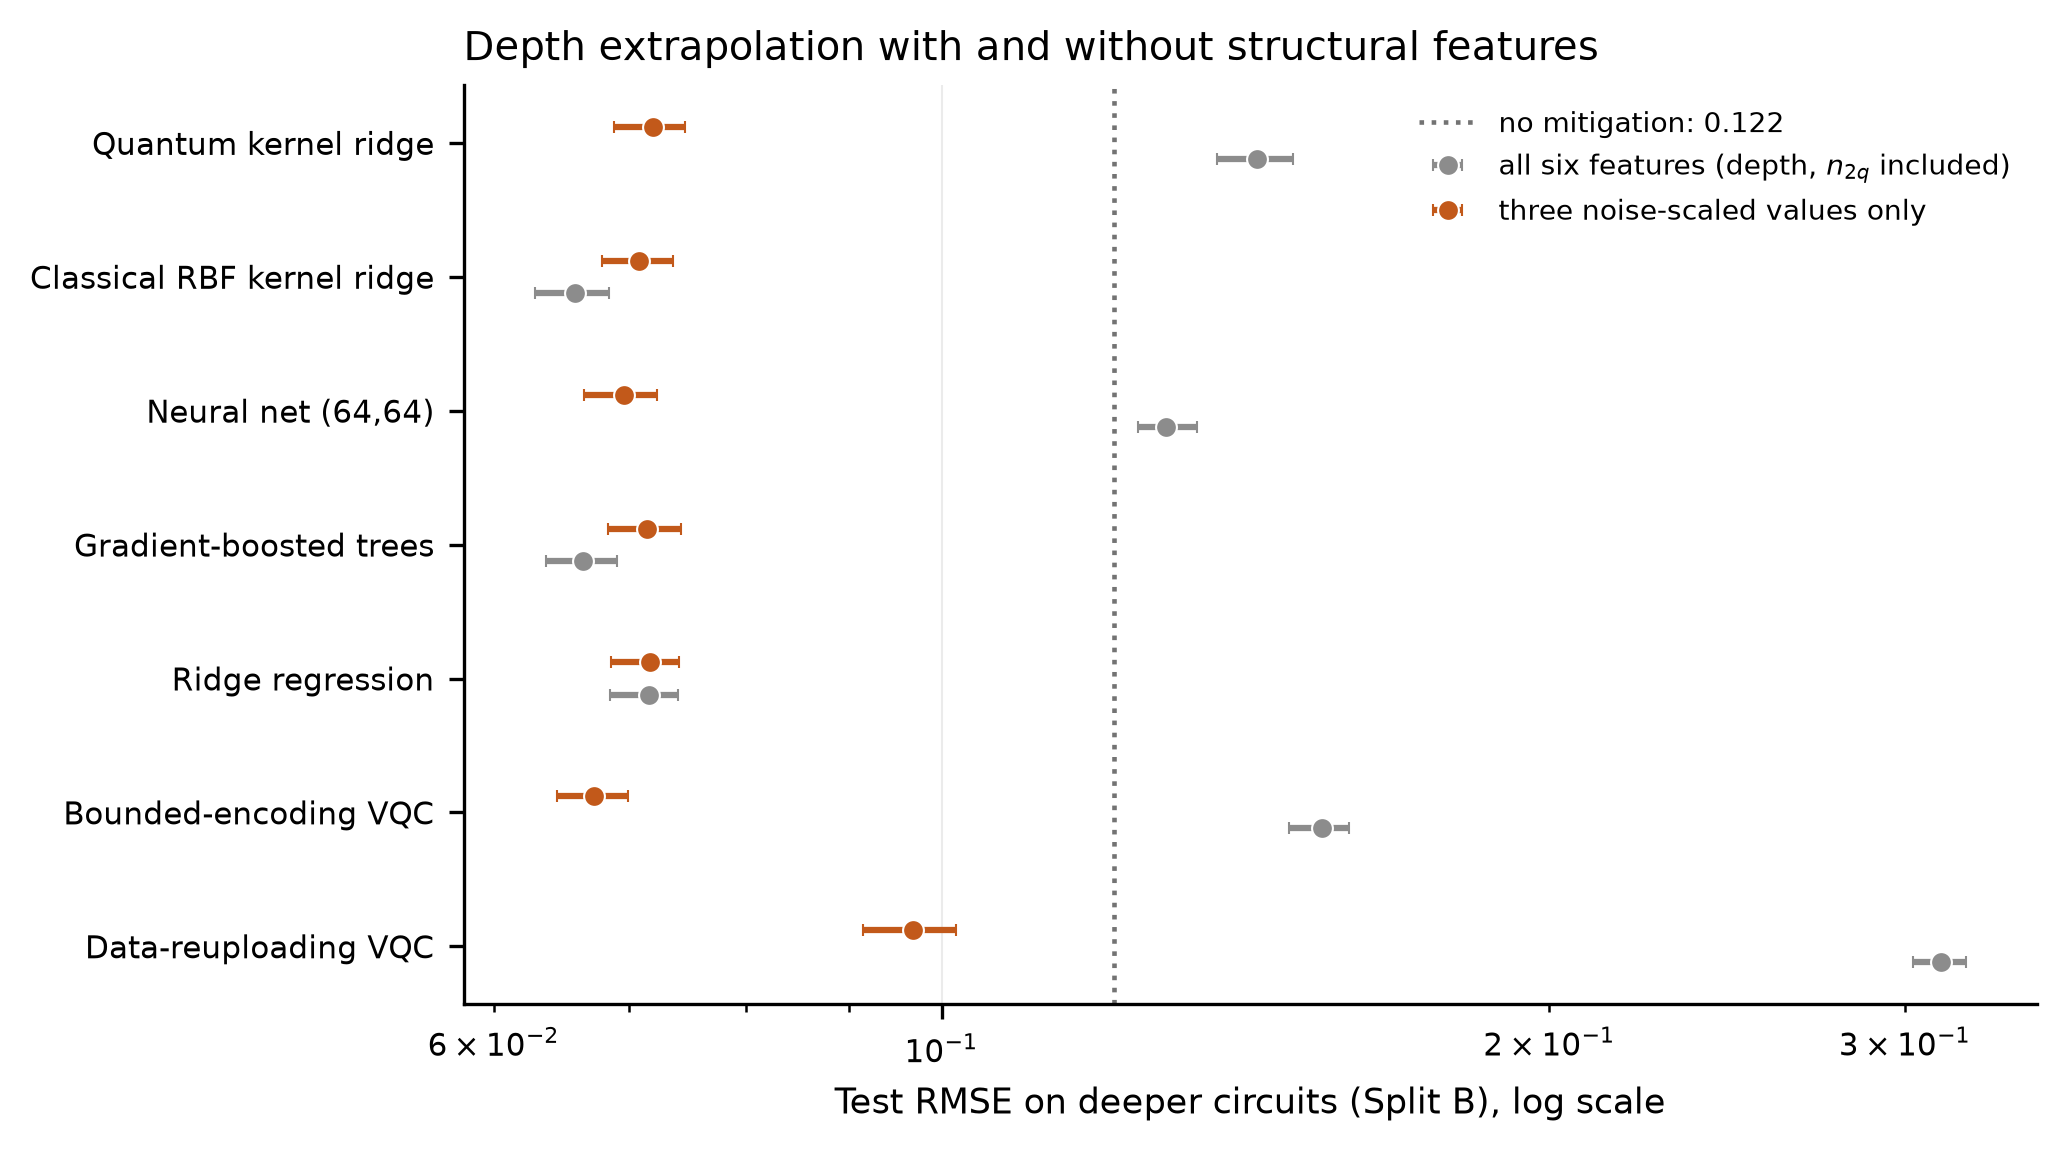
\includegraphics[width=0.85\textwidth]{figures/ch5/fig_ch5_ood_features.png}
\caption[Depth extrapolation with all inputs or noise-scaled inputs]{Depth
extrapolation with all six inputs or the three noise-scaled values alone.
The scale is logarithmic, bars are $95\%$ bootstrap intervals, and the dotted
line marks the unmitigated RMSE.}
\label{fig:ch5_oodfeat}
\end{figure}

Removing depth and two-qubit gate count while keeping observable weight
increases RBF's RMSE from $0.0658$ to $0.0718$ and lowers fidelity RMSE from
$0.1433$ to $0.0723$. Removing observable weight as well gives $0.0709$ and
$0.0720$, respectively. These refits change the inputs and reduce the width
of the fidelity feature map. They measure sensitivity to the choice of
feature set on this depth split.

\section{Summary of findings, idealised regime}\label{sec:ch5_summary}

The matched classical control reaches $0.0404$ RMSE on random held-out
circuits and $0.0658$ on deeper circuits. The fidelity
kernel reaches $0.0421$ and $0.1433$,
respectively. The ablations and learning curves show how the comparison
depends on the features and on the number of reference circuits. The separate seed study shows that the data-reuploading VQC is sensitive to initialisation.

\section{Trace-distance revivals in the device-informed model}
\label{sec:ch5_nonmarkov}

Figure~\ref{fig:ch5_nonmarkov} applies the Breuer--Laine--Piilo trace-distance
diagnostic of Section~\ref{sec:ch3_blp} to qubit $q_0$ during fourteen idle
layers. With the defect coupled, the trace distance for the computational-basis
probe pair falls from $0.907$ at the first idle layer to $0.015$ at the fifth
and revives to $0.896$ at the tenth. This increase witnesses information
backflow for the tested idle evolution. The maximum total revival across the
two tested probe pairs is $\mathcal{N}_{\mathrm{probe}}=0.88$.

Both controls show zero revival for the same probes and idle window. The
defect-removed control decouples the defect. The reset control preserves the
collision and damping parameters and returns the defect to its ground state
between layers. Its first-layer trace distance matches production. In a separate
twelve-layer sweep, the finite-probe statistic gives $0$, $0$, $0.57$, $0.88$,
$1.70$ and $2.70$ at $g=0$, $0.05$, $0.10$, $0.15$, $0.25$ and $0.40$~rad,
respectively. A zero means that the sampled trace distances show no revival
in the sweep window.

\begin{figure}[htbp]
\centering
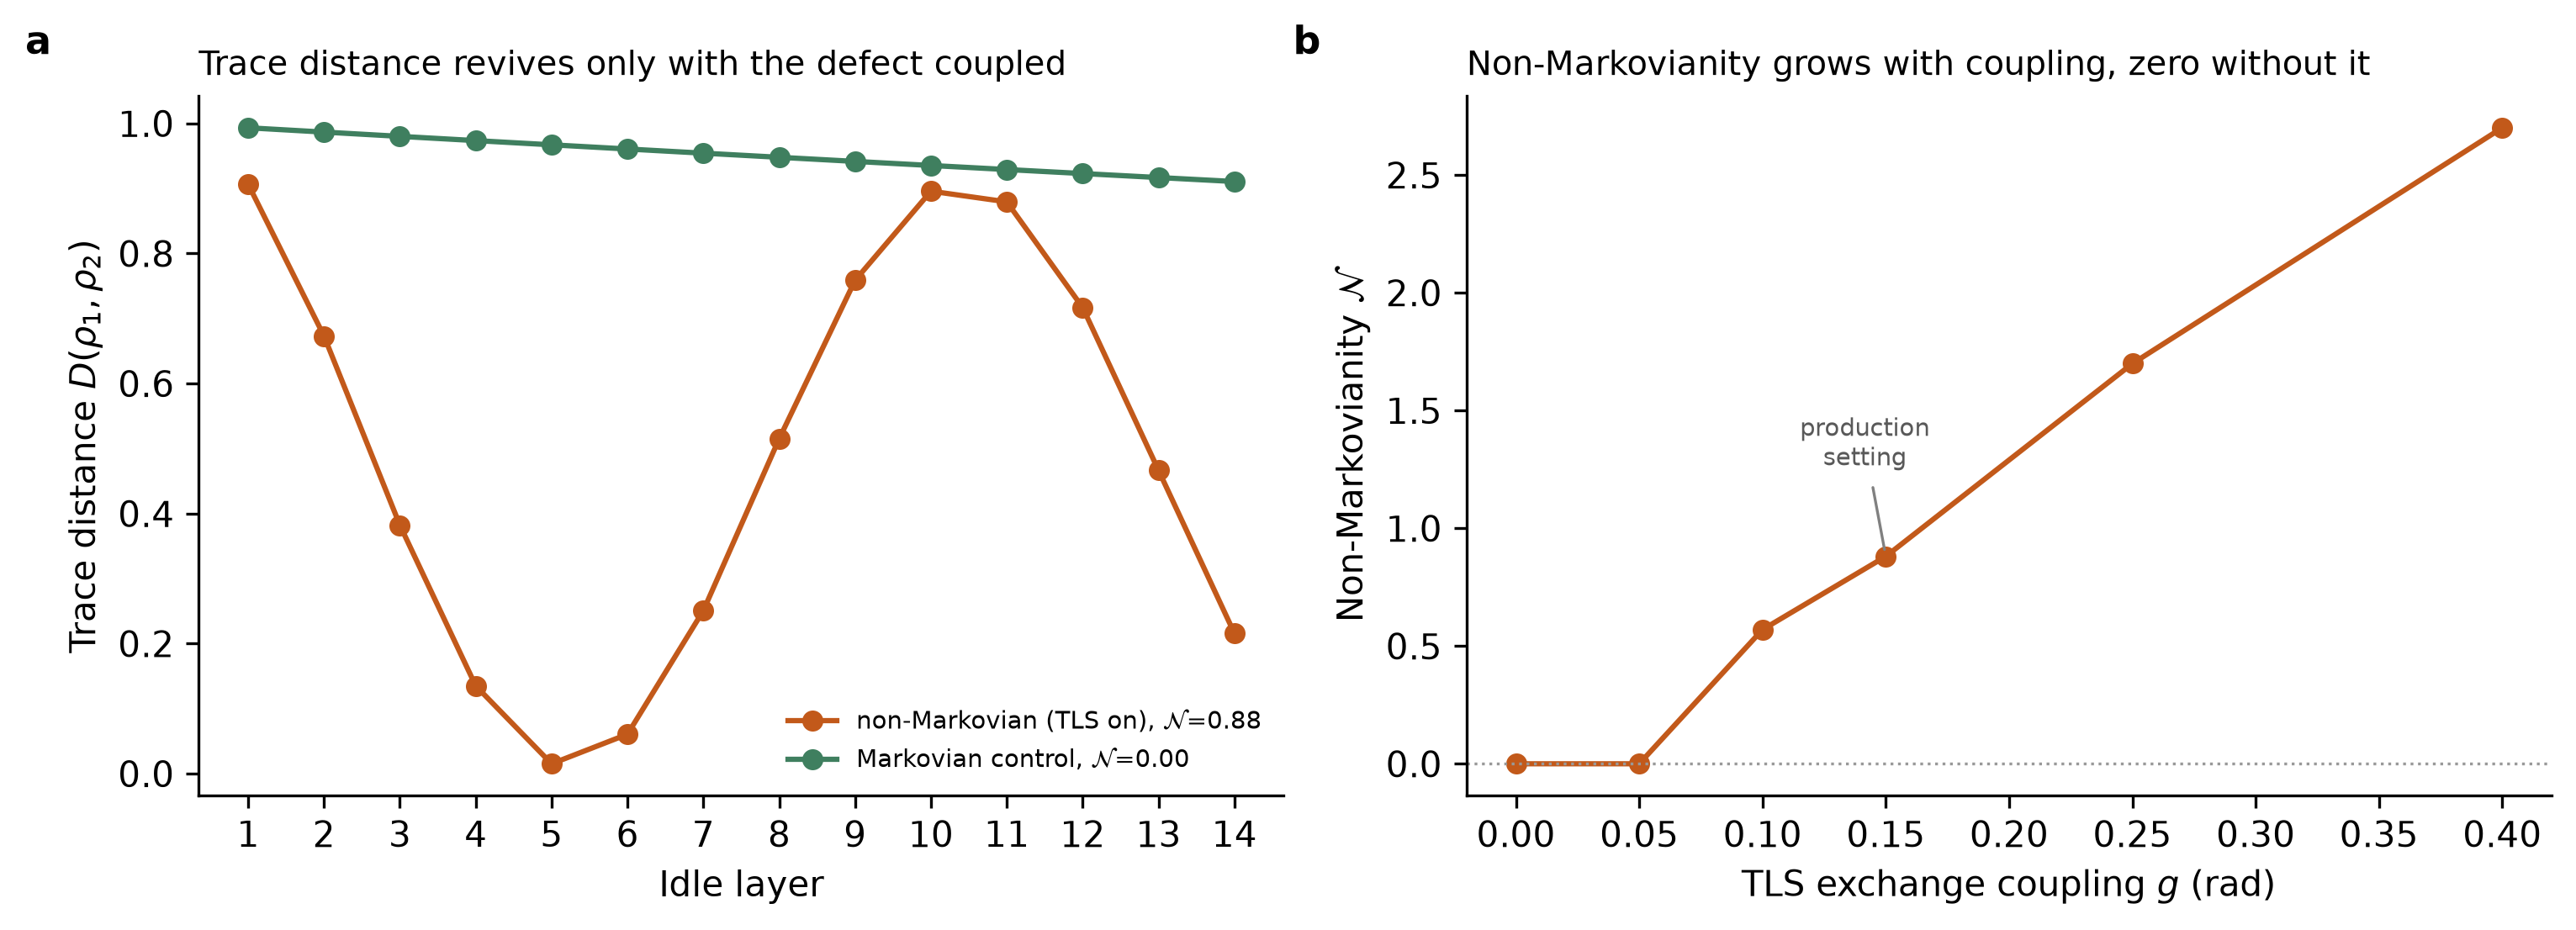
\includegraphics[width=\textwidth]{figures/ch5/fig_ch5_nonmarkov.png}
\caption[Idle trace-distance revivals with a coupled defect]{Panel~a shows the
trace distance on $q_0$ across fourteen idle layers for the computational-basis
probe pair in production and with the defect removed. Panel~b shows the maximum
total revival over the two tested probe pairs in the twelve-layer coupling
sweep, labelled $\mathcal{N}$ in the plot.}
\label{fig:ch5_nonmarkov}
\end{figure}

Across the $4500$ circuit--observable pairs, the mean absolute deviation of the
unmitigated native measurement is $0.0603$ with the defect removed, $0.0870$
with the defect reset between layers, $0.0877$ in production and $0.0930$ after
drift. Most of the difference between production and defect removal persists
when the defect is reset between layers. The production-minus-reset contrast
measures the effect of that intervention with the collision parameters fixed.

\section{Parameter scaling versus unitary folding}\label{sec:ch5_scaling}

Table~\ref{tab:ch5_scaling} and Figure~\ref{fig:ch5_scaling} compare the
two scaling protocols on identical circuits and grouped splits in the
reference production pool. The
tuning budget is fixed across protocols, with $24$ candidates per
kernel. Both use the same $4096$ scale-1 shots per circuit--observable pair.
The three folded ZNE fits use the realised layer ratio for each observation
(Eq.~\eqref{eq:ch3_fold_ratio}). The middle coordinate is $7/3$ at depth
$3$ and $9/5$ at depth $5$. These depths account for $520$ of the $1350$
test rows on Split~A and $920$ of the $1755$ test rows on Split~B.
The noiseless folding test verifies that the
folded circuits preserve the ideal expectation values to
$3.9 \times 10^{-16}$ (Section~\ref{sec:ch4_verification}).

\begin{table}[htbp]
\centering
\caption[Parameter scaling against unitary folding, realistic regime]{Parameter
scaling and unitary folding under production noise. The unmitigated
observation is shared. The last column gives the paired difference
RMSE(folding) $-$ RMSE(parameter) on Split~A and its $95\%$ interval.
An asterisk marks a resolved difference.}
\label{tab:ch5_scaling}
\small
\setlength{\tabcolsep}{5pt}
\begin{tabular}{lccccc}
\toprule
& \multicolumn{2}{c}{\textbf{Split A}} & \multicolumn{2}{c}{\textbf{Split B}} & \\
\cmidrule(lr){2-3} \cmidrule(lr){4-5}
\textbf{Method} & \textbf{Param.} & \textbf{Folding} & \textbf{Param.} & \textbf{Folding}
& \textbf{$\Delta$ Split A} \\
\midrule
Classical RBF kernel ridge & 0.0622 & 0.0762 & 0.0834 & 0.1031 & $+0.014\,[0.009, 0.019]^{*}$ \\
Quantum kernel ridge & 0.0622 & 0.0757 & 0.0878 & 0.1025 & $+0.013\,[0.008, 0.019]^{*}$ \\
Neural net (64,64) & 0.0648 & 0.0798 & 0.1357 & 0.1424 & $+0.015\,[0.010, 0.020]^{*}$ \\
Ridge regression & 0.0673 & 0.0830 & 0.0912 & 0.1104 & $+0.016\,[0.011, 0.021]^{*}$ \\
Gradient-boosted trees & 0.0708 & 0.0834 & 0.0903 & 0.1039 & $+0.013\,[0.007, 0.018]^{*}$ \\
Bounded-encoding VQC & 0.0728 & 0.0907 & 0.1080 & 0.1879 & $+0.018\,[0.014, 0.022]^{*}$ \\
ZNE, linear & 0.1023 & 0.0902 & 0.1253 & 0.1218 & $-0.012\,[-0.015, -0.009]^{*}$ \\
ZNE, Richardson (deg 2) & 0.1201 & 0.2001 & 0.1076 & 0.1963 & $+0.080\,[0.064, 0.096]^{*}$ \\
No mitigation & 0.1239 & 0.1239 & 0.1370 & 0.1370 & $0\,[0, 0]$ \\
Data-reuploading VQC & 0.1511 & 0.0924 & 0.1120 & 0.1542 & $-0.059\,[-0.071, -0.046]^{*}$ \\
ZNE, exponential & 0.2074 & 0.1870 & 0.2022 & 0.2014 & $-0.020\,[-0.047, 0.005]$ \\
\bottomrule
\end{tabular}
\end{table}

\begin{figure}[htbp]
\centering
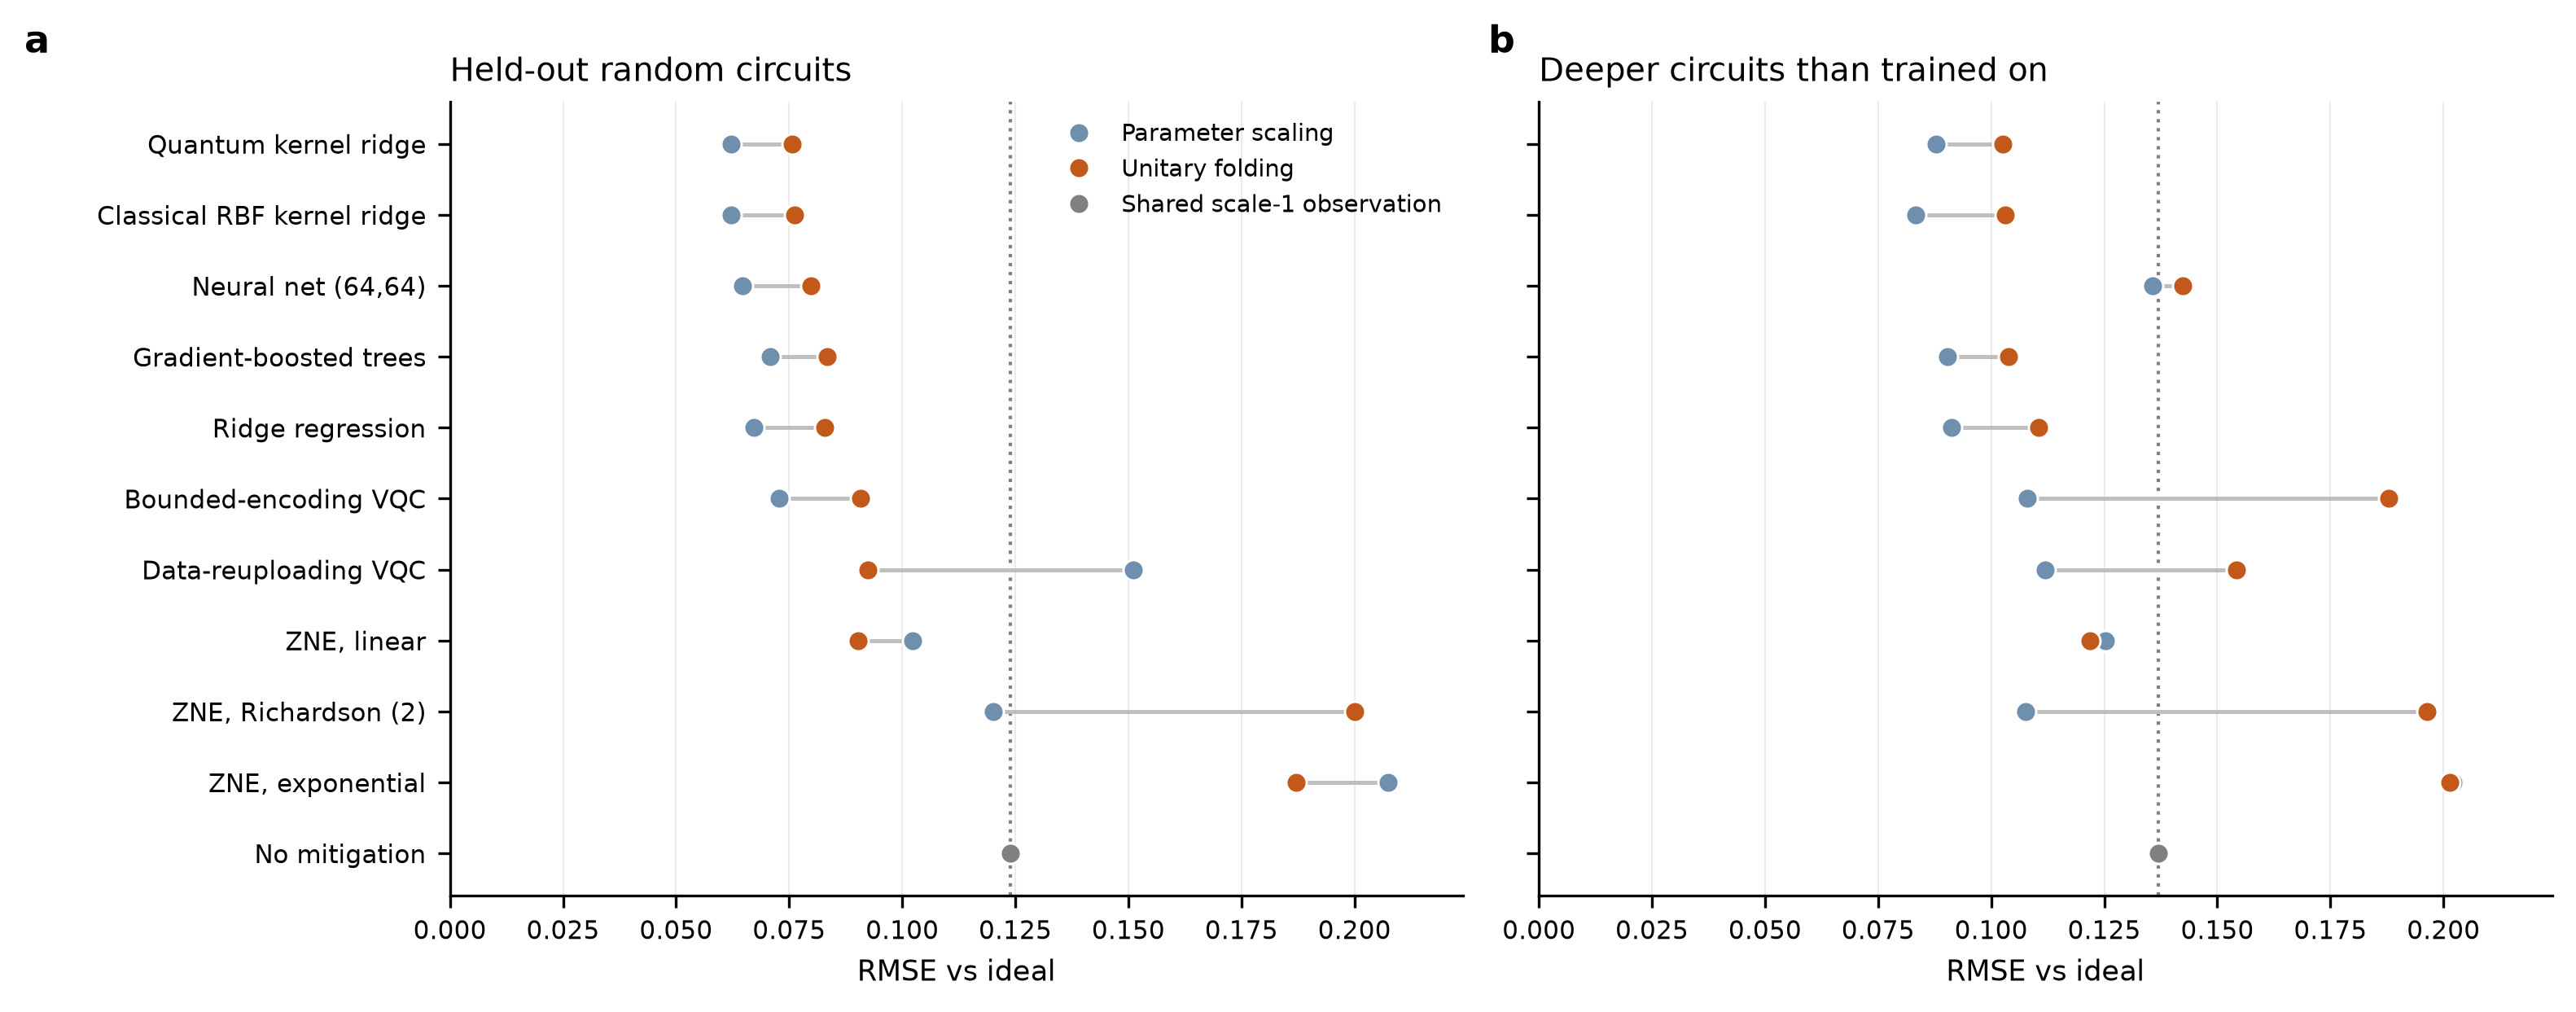
\includegraphics[width=\textwidth]{figures/ch5/fig_ch5_scaling.png}
\caption[Parameter scaling against unitary folding, realistic regime]{Parameter scaling against unitary folding in the realistic regime, on
held-out random circuits (panel~a) and deeper circuits (panel~b). The dotted line
marks the unmitigated RMSE shared by both protocols.}
\label{fig:ch5_scaling}
\end{figure}

On Split~A, both learned kernels have higher RMSE under folding.
RBF goes from $0.0622$ to $0.0762$ and fidelity goes from $0.0622$
to $0.0757$. Linear ZNE improves from $0.1023$ to $0.0902$.
The kernels' RMSE gap below linear ZNE narrows from about $0.040$
with parameter scaling to $0.014$ with folding. On this reference pool,
both kernels have lower RMSE than linear ZNE on both holdouts under
both protocols, with paired intervals excluding zero. Richardson ZNE worsens from $0.1201$
to $0.2001$ on Split~A.

On the random split, the paired RBF-minus-fidelity interval includes zero
under both protocols. On the depth split, the difference
under parameter scaling is $-0.00438$ (95\% CI $[-0.00528,\allowbreak -0.00347]$).
Under folding, RBF and fidelity reach $0.1031$ and $0.1025$.
Their paired difference is $+0.00059$ (95\% CI
$[-0.00158,\allowbreak +0.00289]$).

\section{Replication of the scaling comparison across circuit pools and shot draws}
\label{sec:ch5_folding_seeds}

The scaling comparison was repeated under the reference production calibration on
three independently generated pools of $900$ circuits. Each pool contains
$450$ HEA and $450$ TFIM circuits with five observables per circuit. The
circuit generator used seeds $2026112501$ through $2026112503$. For each pool,
the exact expectations were computed once and used to simulate three
independent sets of $4096$-shot observations per setting. The shot seed labels
$2026112511$ through $2026112513$ were each combined with the circuit seed
using NumPy's \texttt{SeedSequence} to initialise a separate shot stream per
seed combination. The protocols shared one native-scale draw in each
combination, and the folded extrapolators used the executed layer ratios.

The eleven mitigation arms were evaluated for every seed combination under
both scaling protocols. Within a pool, Split~A used the same $70/30$
circuit-grouped holdout with seed~$7$, and Split~B trained on circuits at
depth $\leq4$ and tested at depth $\geq5$. Split~A tested $270$ circuits
per pool. Split~B tested $346$, $375$ and $341$ circuits in seed order.
Both protocols reused these partitions for all shot draws in each pool.
The learned arms were refit in each combination using the reference
training budgets and the same six features. The kernels tuned on four
matched circuit-grouped inner folds with $24$ candidates each.
Each $95\%$ interval compares methods or protocols on the same test
circuits within one seed combination. The nine combinations share circuits
within each of three pools, so the interval counts describe the observed
replications. Across-pool variation is summarised by the range of the three
pool means, each averaged over its shot draws.

Linear ZNE has lower RMSE with folding in all nine combinations on each
split, with paired intervals excluding zero. Folded minus parameter-scaled
RMSE averages $-0.00942$ on Split~A and $-0.00387$ on Split~B. The observed
ranges are $[-0.01033,\allowbreak -0.00901]$ and
$[-0.00470,\allowbreak -0.00291]$, respectively. The unmitigated RMSE is
identical between the two protocols in each combination because the native
shots are shared.

Richardson ZNE has higher RMSE with folding in all seed combinations,
with mean increases of $0.07287$ and $0.08112$ on Splits~A and~B.
Figure~\ref{fig:ch5_foldingseed_scaling} shows the change in error for all
eleven arms.

\begin{figure}[htbp]
\centering
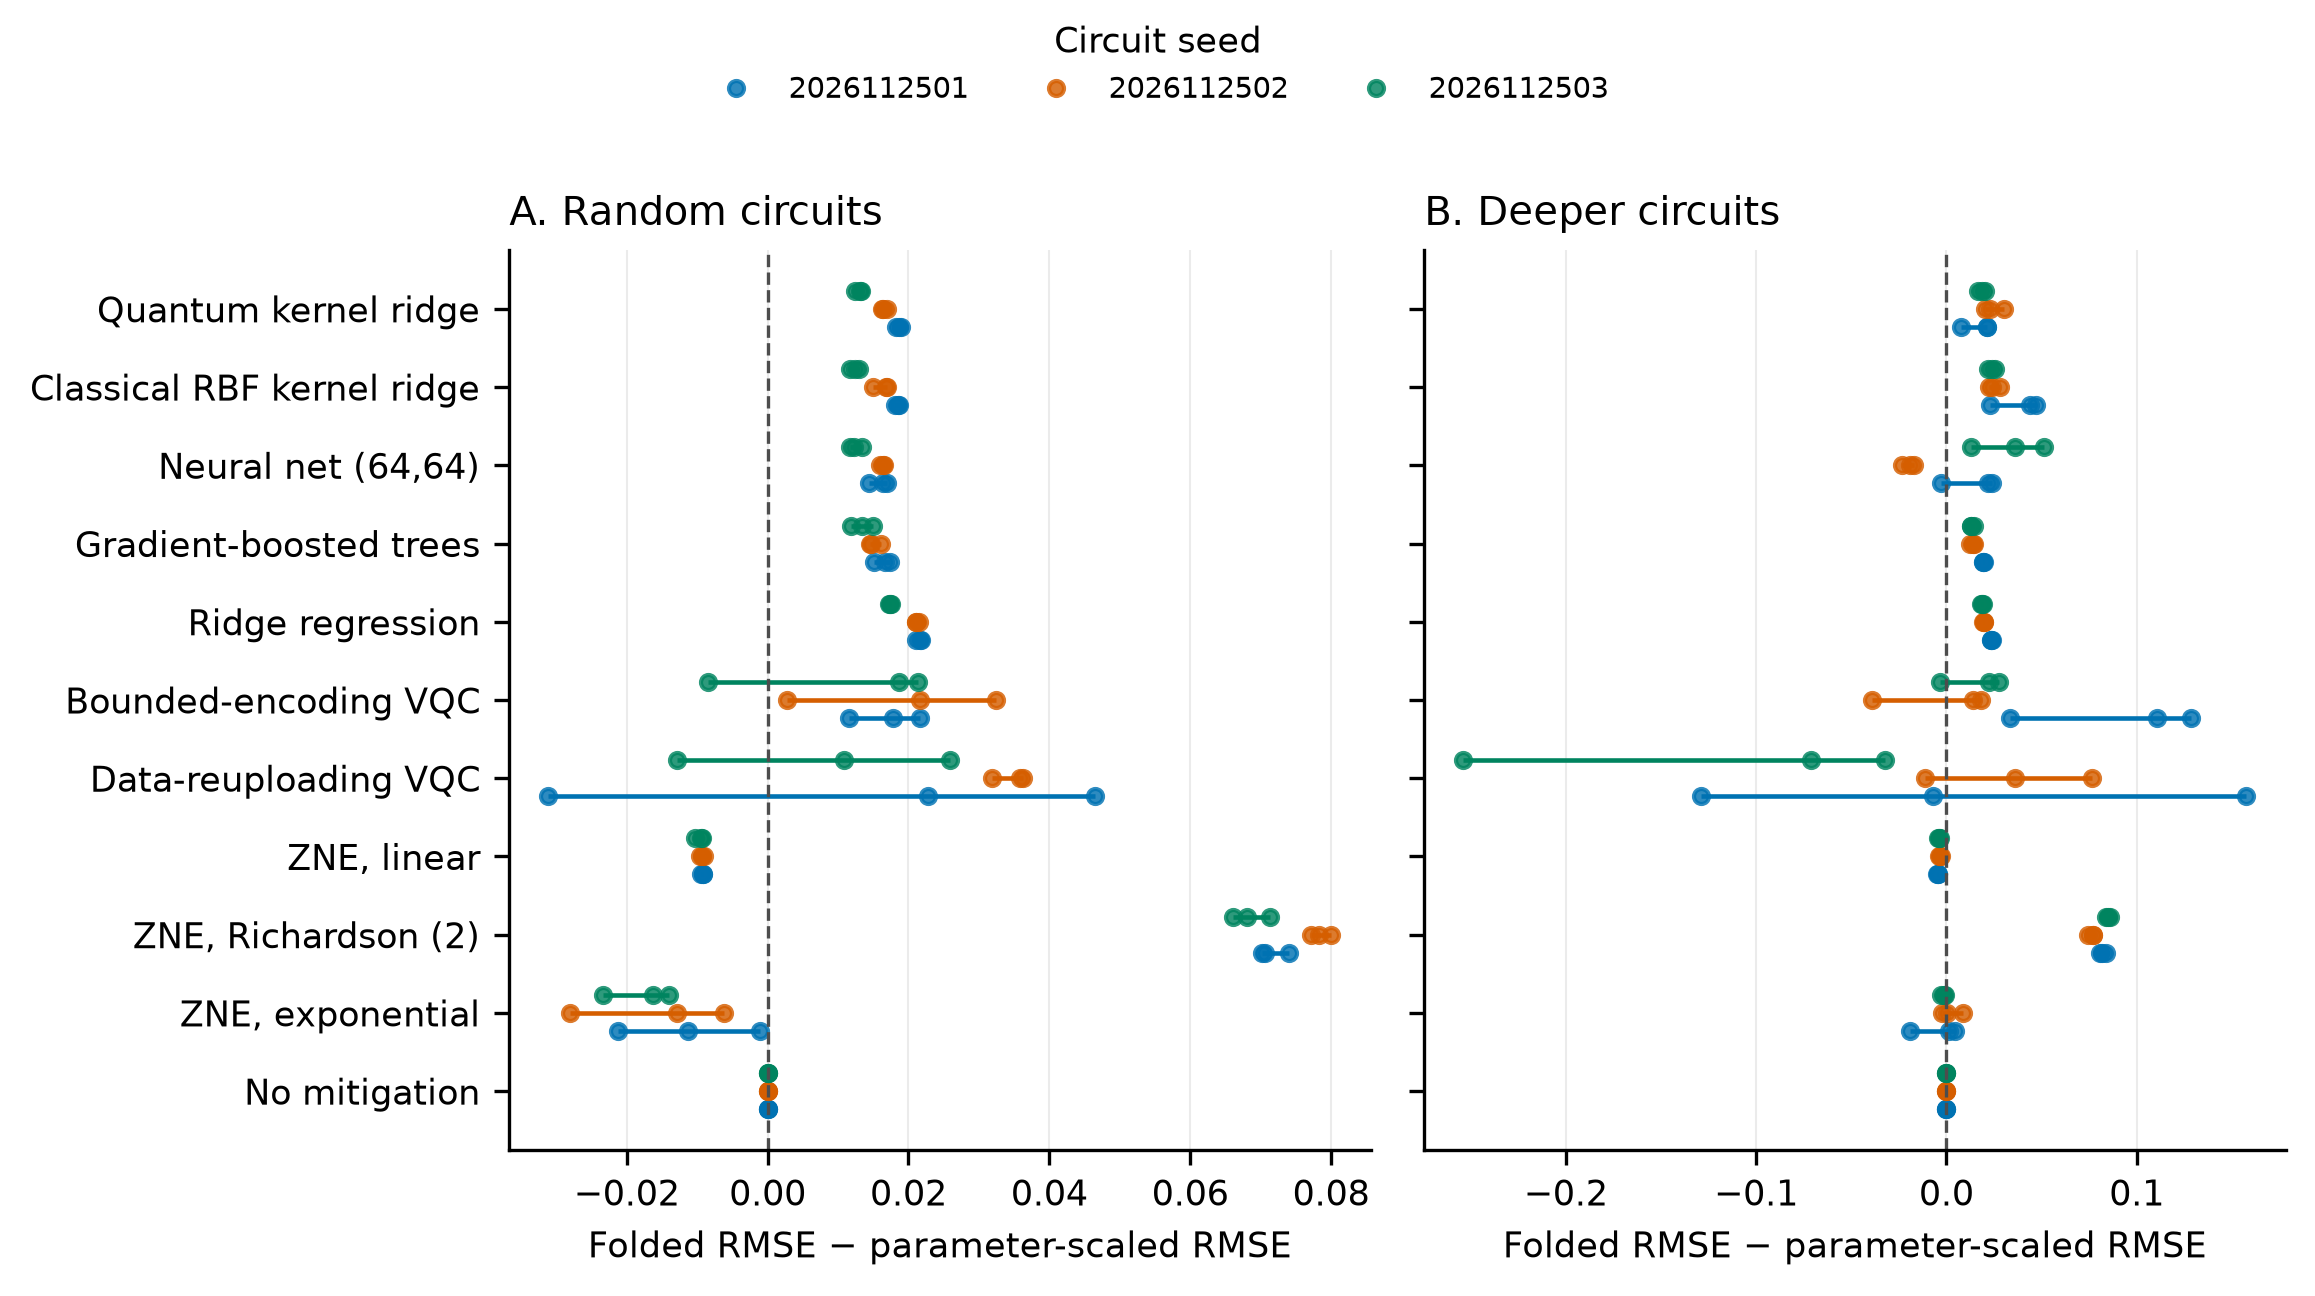
\includegraphics[width=\textwidth]{figures/ch5/fig_ch5_folding_seed_scaling.png}
\caption[Scaling differences over circuit and shot seeds]{The paired change in
test RMSE from parameter scaling to folding. Each marker is a circuit-pool and
shot-draw combination. Colours identify pools and horizontal segments span the
three shot draws in each pool. Negative values favour folding. The panels use
different horizontal scales.}
\label{fig:ch5_foldingseed_scaling}
\end{figure}

Both kernels have higher RMSE under folding than under parameter scaling,
with paired intervals excluding zero in all nine combinations on each
split. On random circuits, both kernels beat folded linear ZNE in all nine
combinations. On deeper circuits, paired intervals favour fidelity over folded
linear ZNE in all nine combinations and favour RBF over folded linear ZNE in seven.
The other two RBF intervals include zero. Among the
eleven arms, gradient-boosted trees give the lowest mean folded depth RMSE
of $0.1036$.

\begin{table}[htbp]
\centering
\caption[Kernel comparison over circuit and shot seeds]{Mean kernel RMSE
across the nine seed combinations for each scaling protocol and split. The
last three columns count within-combination paired intervals that favour
RBF, favour fidelity or include zero.}
\label{tab:ch5_folding_seed_kernels}
\small
\begin{tabular}{llccrrr}
\toprule
Split & Scaling & RBF RMSE & Fidelity RMSE & RBF & Fidelity & Includes 0 \\
\midrule
A & Parameter scaling & 0.0648 & 0.0652 & 3 & 0 & 6 \\
A & Unitary folding & 0.0805 & 0.0812 & 4 & 0 & 5 \\
B & Parameter scaling & 0.0841 & 0.0869 & 7 & 0 & 2 \\
B & Unitary folding & 0.1131 & 0.1069 & 2 & 4 & 3 \\
\bottomrule
\end{tabular}
\end{table}

Table~\ref{tab:ch5_folding_seed_kernels} and
Figure~\ref{fig:ch5_foldingseed_kernels} show the direct kernel contrasts.
On random circuits the paired intervals favour RBF in three parameter
combinations and four folding combinations. On deeper circuits the
parameter-scaled intervals favour RBF in seven combinations. The folded
depth intervals favour fidelity in four combinations, RBF in two, and
include zero in three. The folded depth mean RBF-minus-fidelity difference
is $+0.00618$, and the three pool means range from $-0.00017$ to $+0.01868$.
Three of the four favourable fidelity intervals are from the pool with
circuit seed $2026112501$. Table~\ref{tab:appB_foldingseeds} reports the
other paired scaling contrasts and their spread.

\begin{figure}[htbp]
\centering
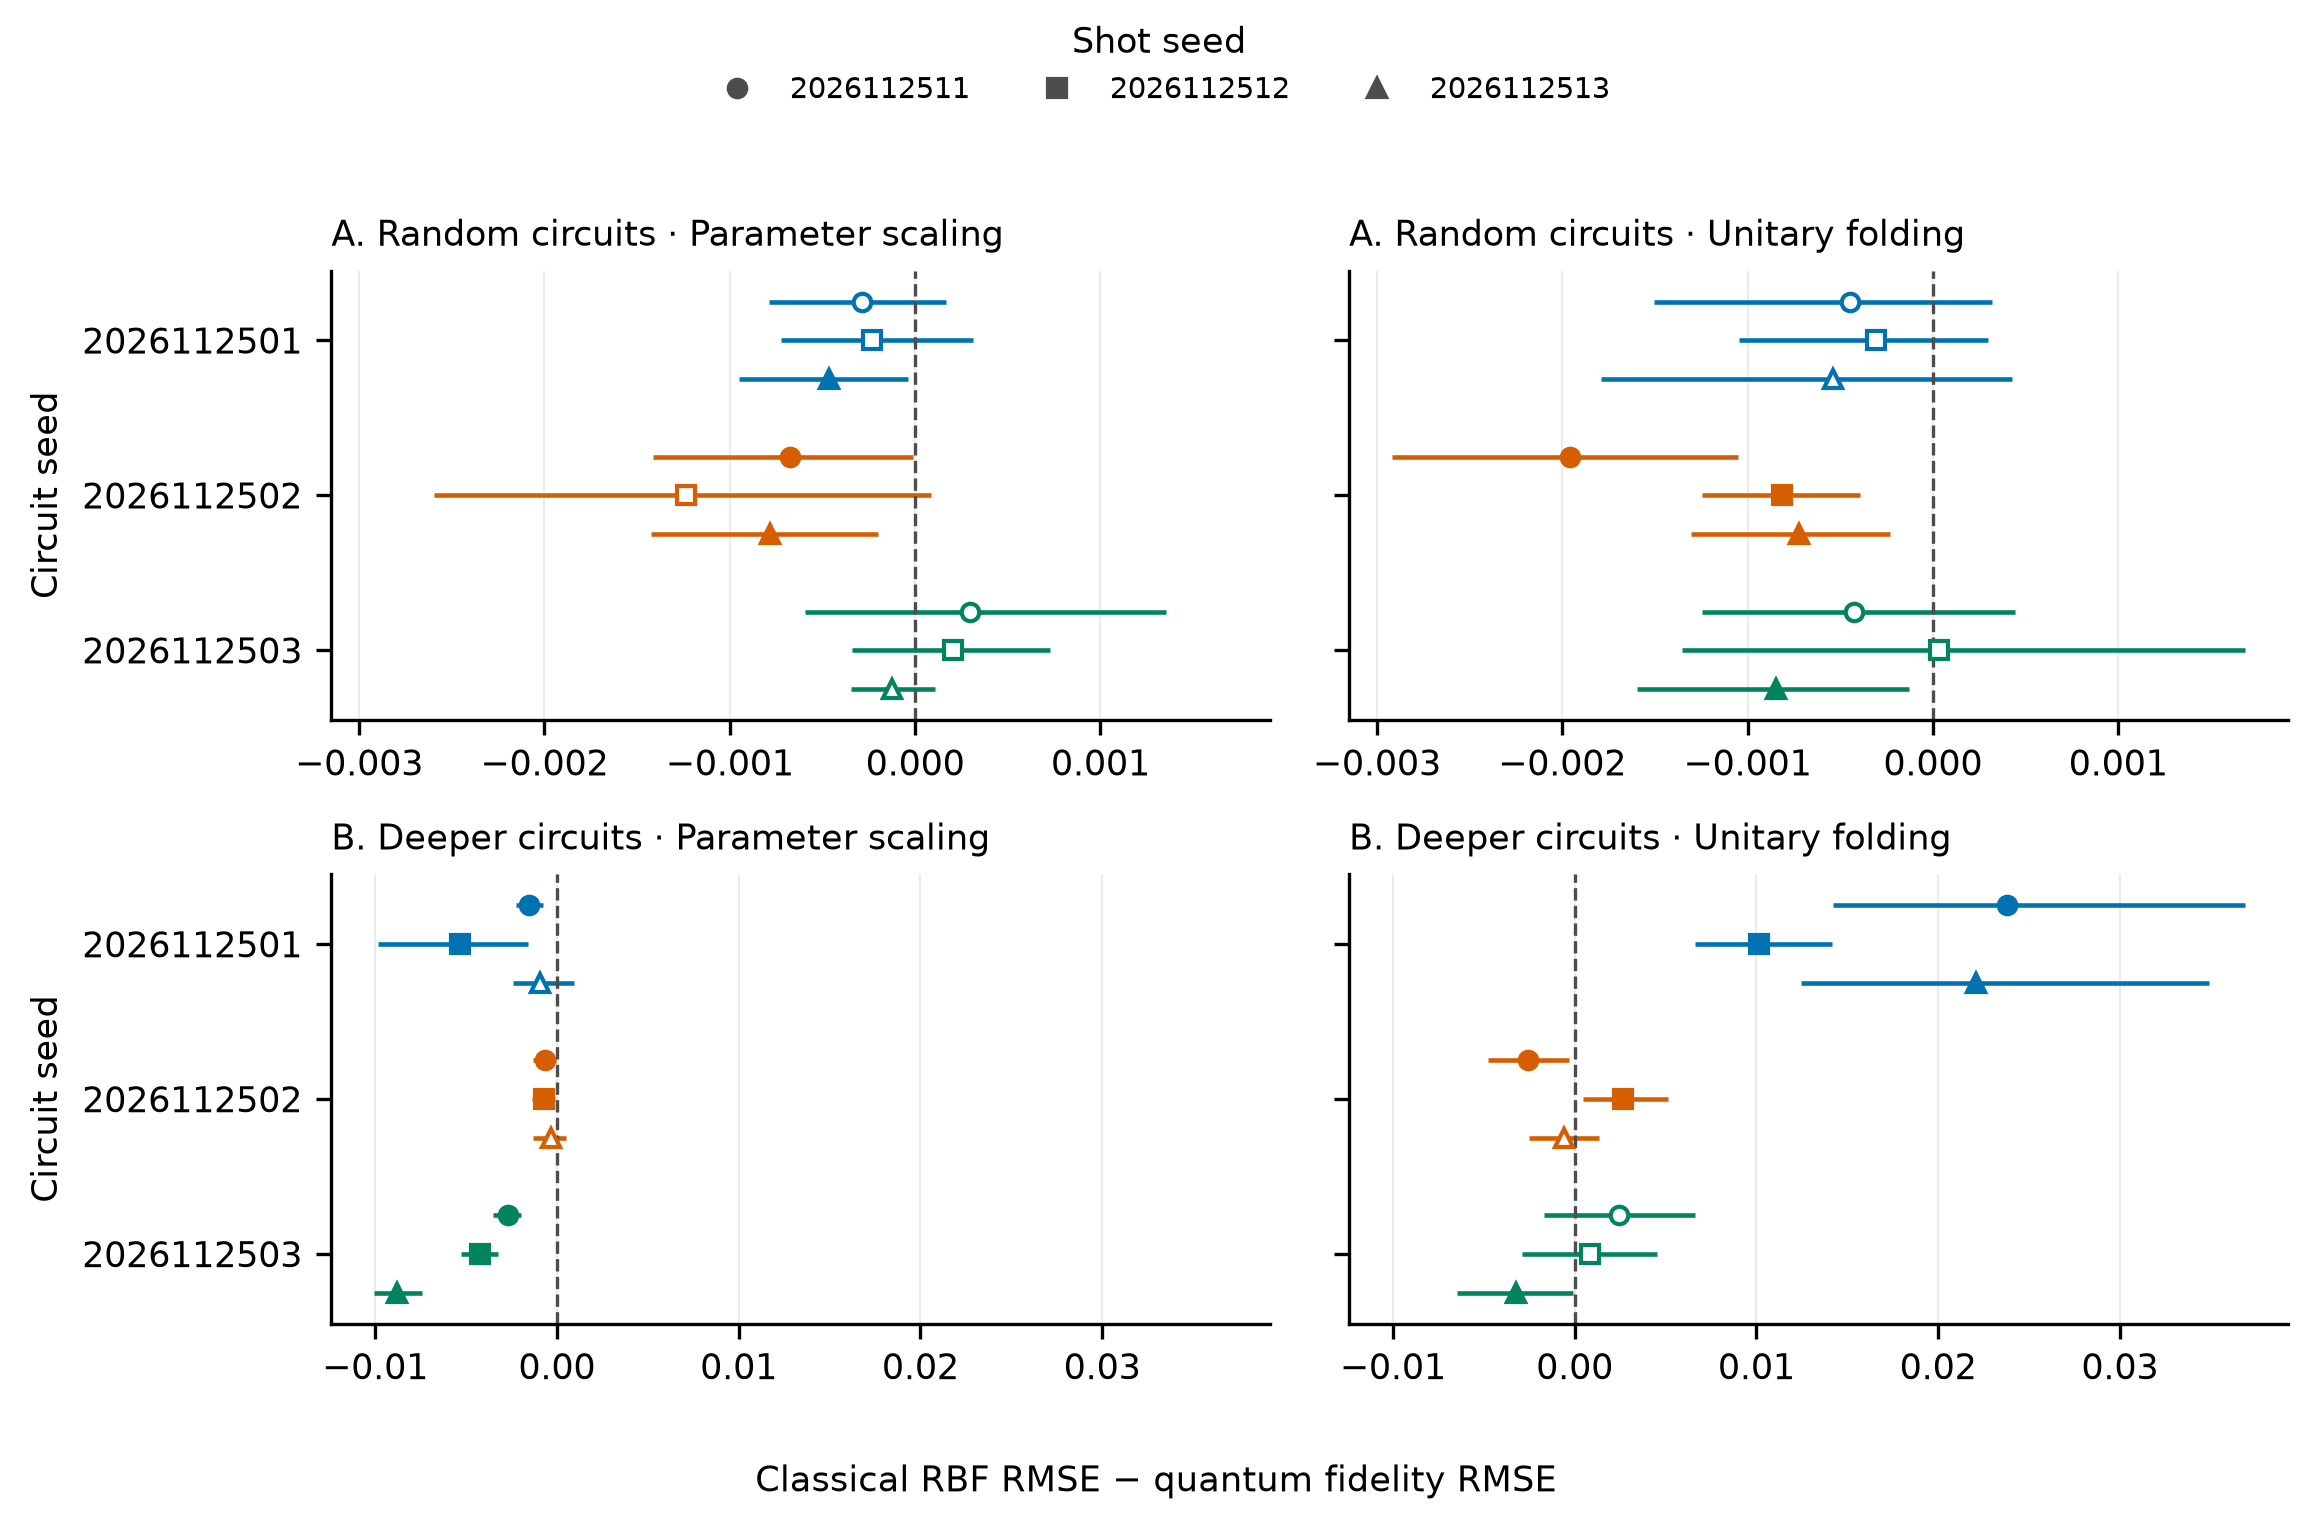
\includegraphics[width=\textwidth]{figures/ch5/fig_ch5_folding_seed_kernels.png}
\caption[Paired kernel comparisons over circuit and shot seeds]{Classical RBF
minus quantum fidelity RMSE for every seed combination. Whiskers show $95\%$
paired circuit-bootstrap intervals within each combination. Filled markers
denote intervals that exclude zero. Negative values favour RBF. Horizontal
scales are shared within each split.}
\label{fig:ch5_foldingseed_kernels}
\end{figure}

\section{Effects of resetting the defect between layers}\label{sec:ch5_markovianity}

Table~\ref{tab:ch5_regime} and Figure~\ref{fig:ch5_regime} compare the production
model with both controls of Section~\ref{sec:ch5_nonmarkov}, under both scaling
methods, on identical circuits. Within each condition, the native-scale
shots are shared by the two protocols. The two $\Delta$ columns compare production with resetting the defect between layers, at fixed collision and damping
parameters.

\begin{table}[htbp]
\centering
\caption[Defect removal and reset controls]{RMSE on Split~A with the defect
removed, reset between layers and in production. $\Delta$ is the paired difference RMSE(production) $-$ RMSE(reset) with its $95\%$ interval, computed from unrounded values. An
asterisk marks a resolved difference.}
\label{tab:ch5_regime}
\resizebox{\textwidth}{!}{%
\begin{tabular}{lcccccccc}
\toprule
& \multicolumn{4}{c}{\textbf{Parameter scaling}} & \multicolumn{4}{c}{\textbf{Unitary folding}} \\
\cmidrule(lr){2-5} \cmidrule(lr){6-9}
\textbf{Method} & \textbf{Removed} & \textbf{Reset} & \textbf{Prod.} & \textbf{$\Delta$}
& \textbf{Removed} & \textbf{Reset} & \textbf{Prod.} & \textbf{$\Delta$} \\
\midrule
Classical RBF kernel ridge & 0.0402 & 0.0527 & 0.0622 & $+0.010\,[0.005, 0.014]^{*}$ & 0.0462 & 0.0552 & 0.0762 & $+0.021\,[0.014, 0.029]^{*}$ \\
Quantum kernel ridge & 0.0404 & 0.0525 & 0.0622 & $+0.010\,[0.006, 0.014]^{*}$ & 0.0460 & 0.0553 & 0.0757 & $+0.020\,[0.013, 0.028]^{*}$ \\
Neural net (64,64) & 0.0417 & 0.0562 & 0.0648 & $+0.009\,[0.004, 0.014]^{*}$ & 0.0477 & 0.0561 & 0.0798 & $+0.024\,[0.017, 0.031]^{*}$ \\
Ridge regression & 0.0424 & 0.0604 & 0.0673 & $+0.007\,[0.003, 0.011]^{*}$ & 0.0504 & 0.0595 & 0.0830 & $+0.023\,[0.017, 0.031]^{*}$ \\
Gradient-boosted trees & 0.0474 & 0.0599 & 0.0708 & $+0.011\,[0.006, 0.016]^{*}$ & 0.0534 & 0.0628 & 0.0834 & $+0.021\,[0.013, 0.028]^{*}$ \\
Bounded-encoding VQC & 0.0533 & 0.0691 & 0.0728 & $+0.004\,[-0.004, 0.010]$ & 0.0543 & 0.0714 & 0.0907 & $+0.019\,[0.013, 0.025]^{*}$ \\
ZNE, linear & 0.0522 & 0.1130 & 0.1023 & $-0.011\,[-0.020, -0.001]^{*}$ & 0.0574 & 0.0857 & 0.0902 & $+0.004\,[-0.002, 0.011]$ \\
ZNE, Richardson (deg 2) & 0.0665 & 0.1086 & 0.1201 & $+0.012\,[0.003, 0.020]^{*}$ & 0.0816 & 0.1383 & 0.2001 & $+0.062\,[0.049, 0.076]^{*}$ \\
No mitigation & 0.0807 & 0.1247 & 0.1239 & $-0.001\,[-0.006, 0.004]$ & 0.0807 & 0.1247 & 0.1239 & $-0.001\,[-0.006, 0.004]$ \\
Data-reuploading VQC & 0.0782 & 0.0860 & 0.1511 & $+0.065\,[0.054, 0.076]^{*}$ & 0.1249 & 0.1107 & 0.0924 & $-0.018\,[-0.028, -0.009]^{*}$ \\
ZNE, exponential & 0.1435 & 0.1866 & 0.2074 & $+0.021\,[-0.006, 0.046]$ & 0.1506 & 0.1531 & 0.1870 & $+0.034\,[0.008, 0.059]^{*}$ \\
\bottomrule
\end{tabular}}
\end{table}

\begin{figure}[htbp]
\centering
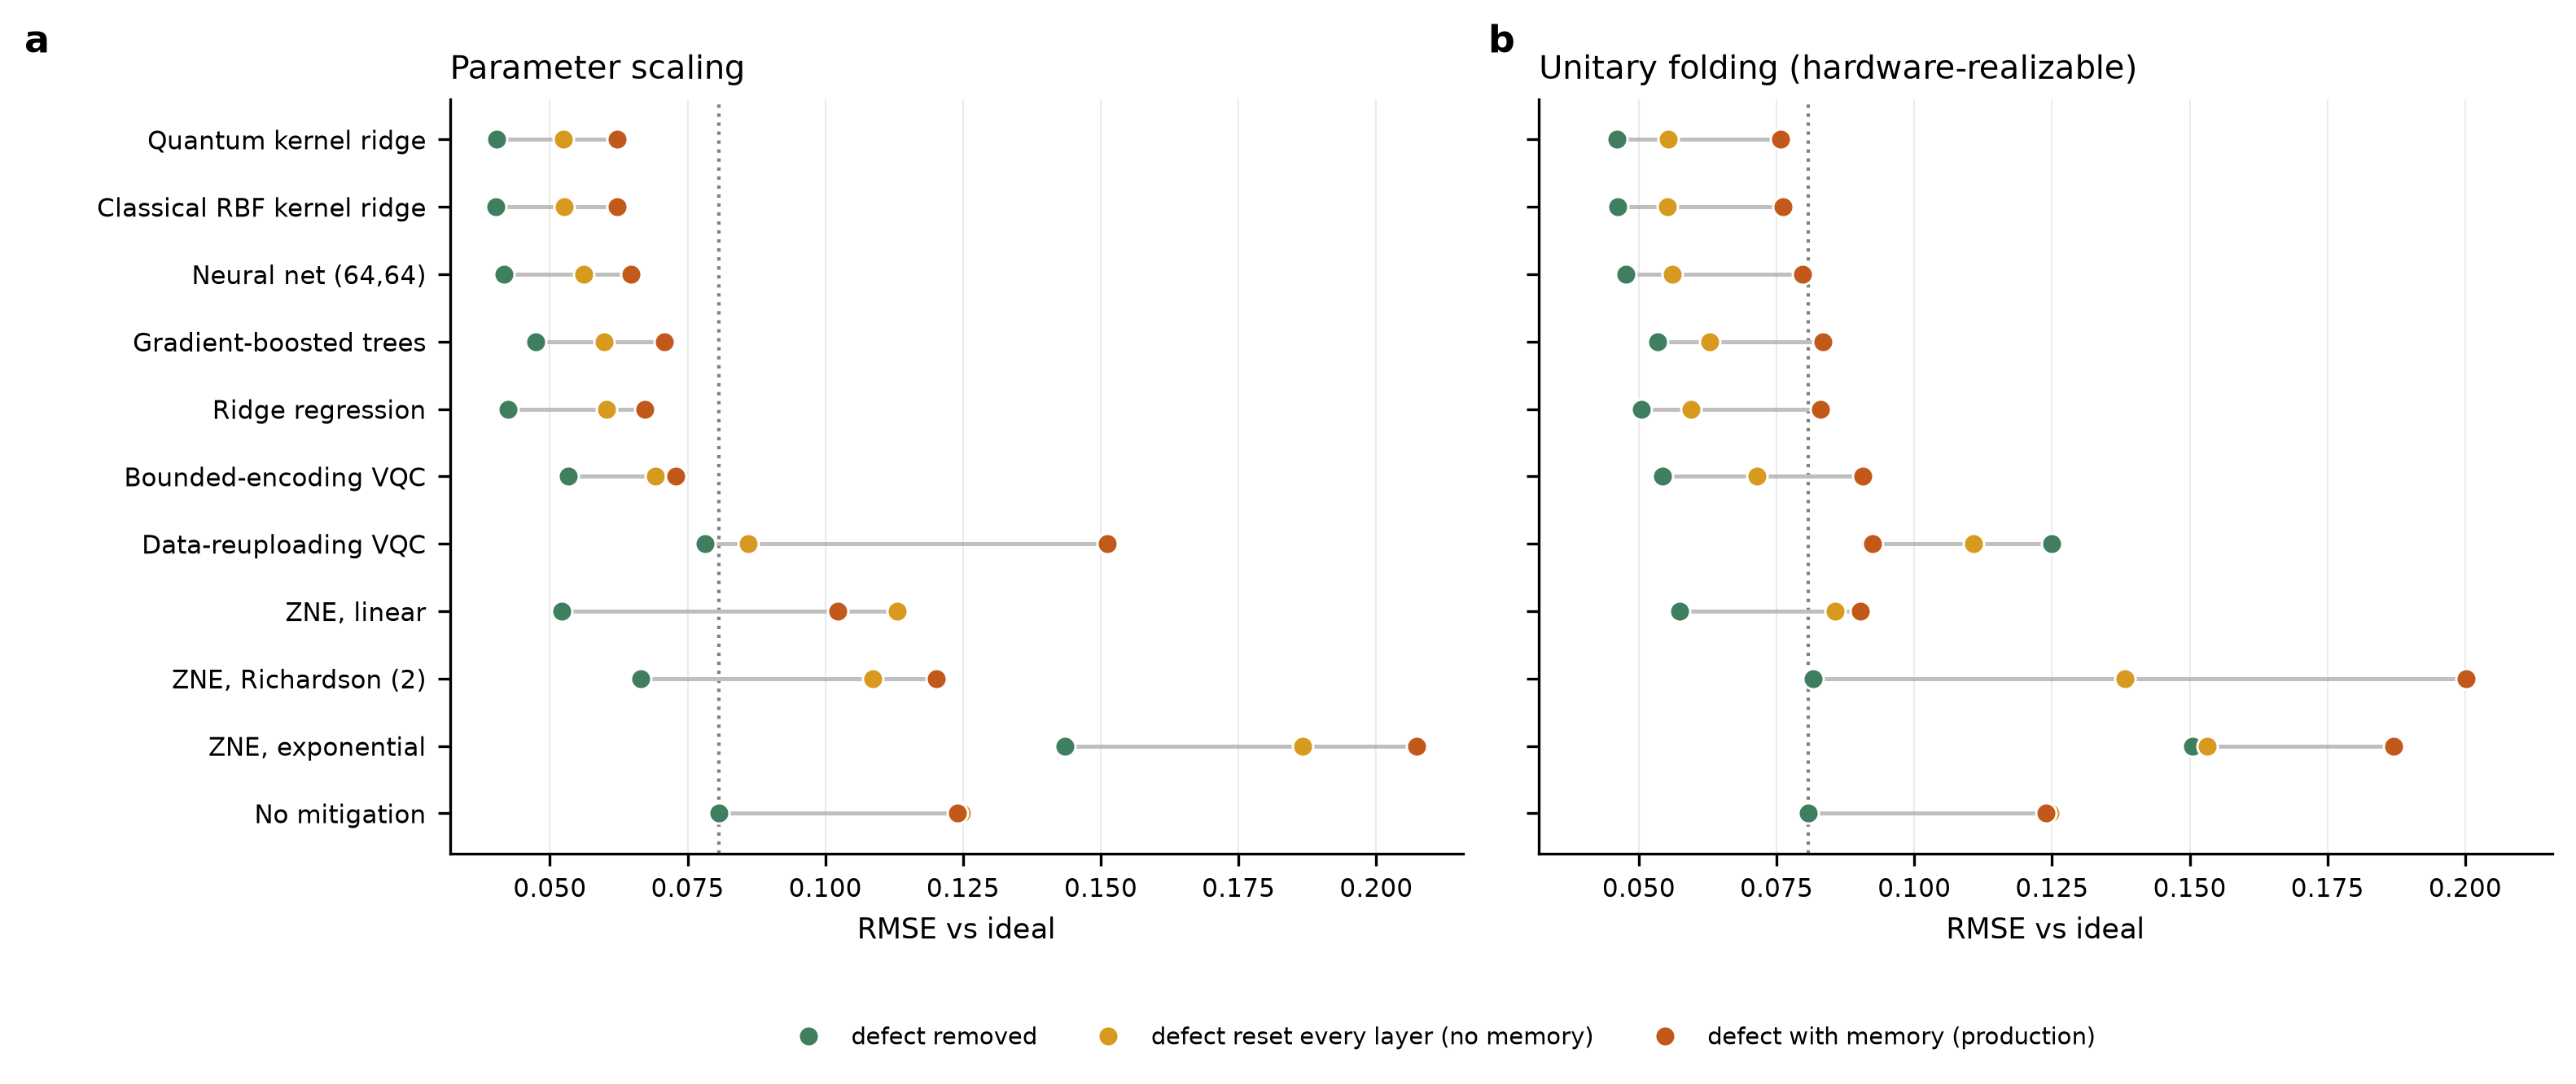
\includegraphics[width=\textwidth]{figures/ch5/fig_ch5_regime.png}
\caption[The cost of the defect under both scaling methods]{The cost of the defect under parameter scaling (panel~a) and unitary
folding (panel~b). Green denotes defect removal, amber denotes a fresh
defect at each layer, and red denotes production with memory. The dotted
line marks the shared unmitigated RMSE with the defect removed.}
\label{fig:ch5_regime}
\end{figure}

Under parameter scaling, the production-minus-reset RMSE differences are
$0.0095$
for RBF and
$0.0098$
for fidelity. Under folding, they are $0.0211$ and $0.0204$,
respectively. All four paired intervals exclude zero
(Table~\ref{tab:ch5_regime}). For folded linear ZNE, the
production-minus-reset interval includes zero.
For the unmitigated estimate, the production-minus-reset interval includes zero
under both scaling methods. The changes in the fitted kernels are specific to
the features and fitted models under this reset intervention.

\section{Calibration drift}\label{sec:ch5_drift}

Table~\ref{tab:ch5_drift} and Figure~\ref{fig:ch5_drift} train every learned arm on
calibration~A and evaluate it after the device has drifted by $30\%$
(calibration~B, Section~\ref{sec:ch3_realistic}), on the same held-out circuits and
on the training circuits themselves. The paired column compares calibration~B with
calibration~A on identical held-out circuits.

\begin{table}[htbp]
\centering
\caption[Calibration drift under parameter scaling]{Calibration drift under parameter scaling. RMSE; $\Delta$ is the paired difference RMSE(B, held-out) $-$ RMSE(A, held-out), computed from unrounded values; an asterisk marks a resolved
difference.}
\label{tab:ch5_drift}
\small
\setlength{\tabcolsep}{4pt}
\begin{tabular}{lcccc}
\toprule
\textbf{Method} & \textbf{A, held-out} & \textbf{B, training} & \textbf{B, held-out}
& \textbf{$\Delta$ drift} \\
\midrule
Classical RBF kernel ridge & 0.0622 & 0.0667 & 0.0635 & $+0.0014\,[-0.0014, 0.0041]$ \\
Quantum kernel ridge & 0.0622 & 0.0666 & 0.0636 & $+0.0014\,[-0.0013, 0.0041]$ \\
Neural net (64,64) & 0.0648 & 0.0666 & 0.0653 & $+0.0005\,[-0.0019, 0.0031]$ \\
Ridge regression & 0.0673 & 0.0740 & 0.0707 & $+0.0034\,[0.0009, 0.0058]^{*}$ \\
Gradient-boosted trees & 0.0708 & 0.0688 & 0.0696 & $-0.0012\,[-0.0045, 0.0022]$ \\
Bounded-encoding VQC & 0.0728 & 0.0762 & 0.0734 & $+0.0005\,[-0.0019, 0.0028]$ \\
ZNE, linear & 0.1023 & 0.1063 & 0.1066 & $+0.0043\,[0.0020, 0.0064]^{*}$ \\
ZNE, Richardson (deg 2) & 0.1201 & 0.1115 & 0.1153 & $-0.0048\,[-0.0093, 0.0001]$ \\
No mitigation & 0.1239 & 0.1263 & 0.1298 & $+0.0059\,[0.0044, 0.0073]^{*}$ \\
Data-reuploading VQC & 0.1511 & 0.1456 & 0.1484 & $-0.0027\,[-0.0083, 0.0036]$ \\
ZNE, exponential & 0.2074 & 0.1941 & 0.1922 & $-0.0152\,[-0.0429, 0.0120]$ \\
\bottomrule
\end{tabular}
\end{table}

\begin{figure}[htbp]
\centering
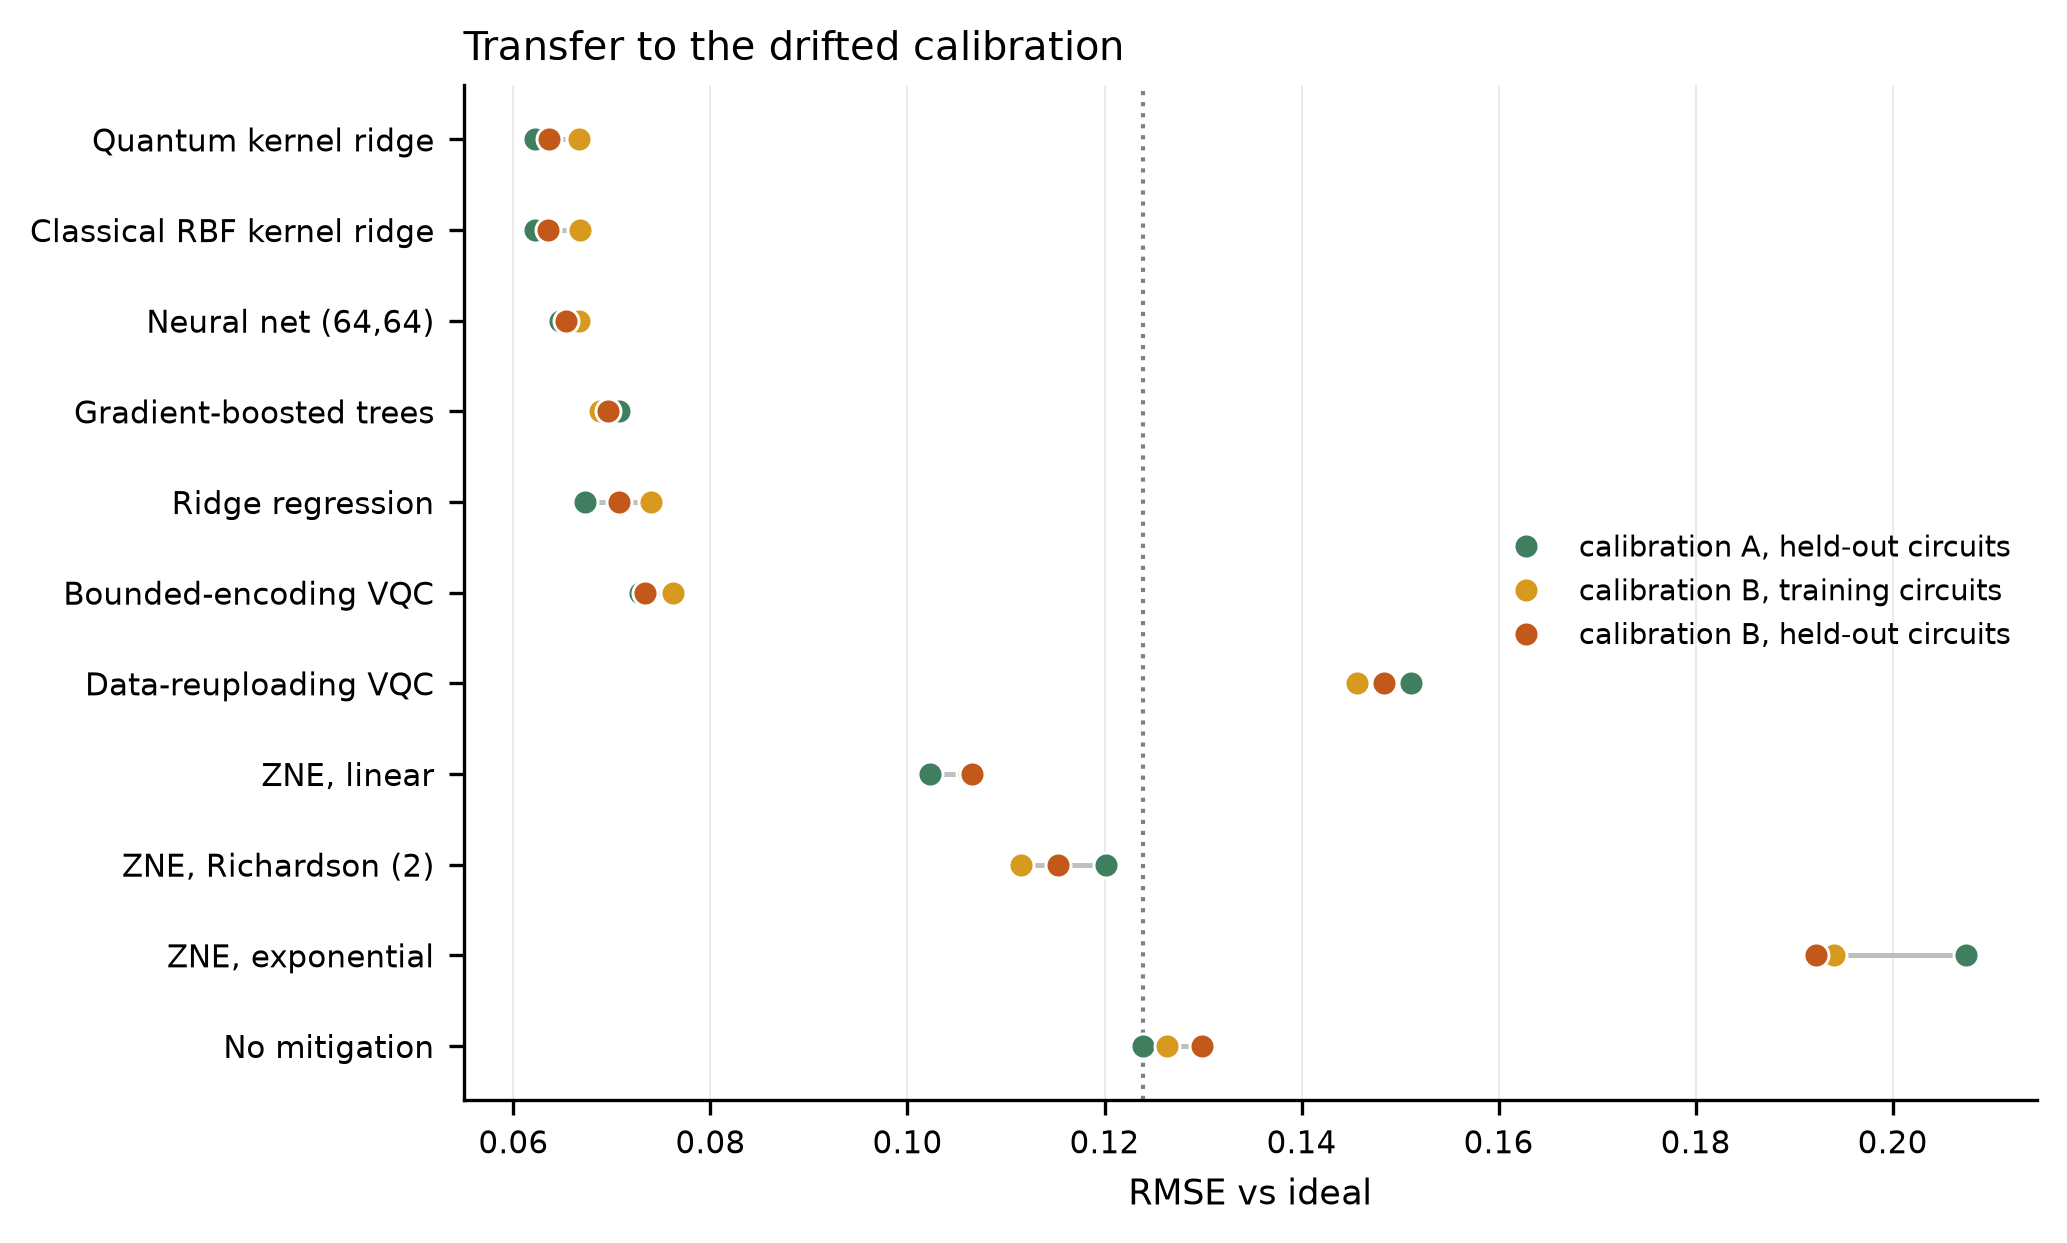
\includegraphics[width=0.85\textwidth]{figures/ch5/fig_ch5_drift.png}
\caption[Calibration drift]{Calibration drift. Each learned arm is trained on calibration~A and
evaluated on calibration~A held-out circuits (green), calibration~B on the training
circuits (amber) and calibration~B on held-out circuits (red).}
\label{fig:ch5_drift}
\end{figure}

For RBF, the difference from calibration~A to calibration~B on the same
held-out circuits is
$+0.00135$ (95\% CI $[-0.00136,\allowbreak +0.00408]$).
For the fidelity kernel it is
$+0.00140$ (95\% CI $[-0.00127,\allowbreak +0.00412]$).
The intervals quantify sensitivity to this drift draw on the simulated device.

\section{Finite-shot fidelity kernels and circuit cost}
\label{sec:ch5_shotkernel}

R4 evaluates the fidelity kernel on the parameter-scaled Split~A of the
realistic regime. Each fidelity entry is estimated by simulating the
binomial shot noise of an inversion test. The simulation uses ideal
inversion-test probabilities and captures sampling variability alone.
For each of the four circuit-grouped inner folds, the feature scaler and
positive semidefinite (PSD) repair are fitted on that fold's training data.
The validation cross-kernel is projected onto the positive eigenspace of
that same training block. After mean validation $R^2$ selects the ridge
penalty, a fresh scaler and repair are fitted on all outer training data.
The final held-out cross-kernel uses the same projection rule
(Eq.~\eqref{eq:appA_shot_projection}). The outer holdout stays fixed
across the five shot-noise draws at each budget.

\begin{table}[htbp]
\centering
\caption[Shot-limited quantum kernel]{Shot-limited fidelity kernel on realistic Split~A.
RMSE is the mean and range over five independent shot draws at each finite budget.
Counts are per draw. Tuning includes the training and validation matrices for all
four inner folds. Final counts the outer training and test matrices. Per prediction
counts the additional fidelity
executions for a new input after fitting. The exact-Gram control uses the same folds,
$\beta=0.15$, projection rule and 12-point $\alpha$ grid with exact fidelities.}
\label{tab:ch5_shotkernel}
\small
\begin{tabular}{lrrrc}
\toprule
\textbf{Shots/entry} & \textbf{Tuning} & \textbf{Final fit/test} & \textbf{Per prediction}
    & \textbf{RMSE (range)} \\
\midrule
$10^{2}$ & $1.86\times 10^{9}$ & $9.22\times 10^{8}$ & $3.15\times 10^{5}$ & 0.0925 (0.0919--0.0933) \\
$10^{3}$ & $1.86\times 10^{10}$ & $9.22\times 10^{9}$ & $3.15\times 10^{6}$ & 0.0740 (0.0735--0.0745) \\
$10^{4}$ & $1.86\times 10^{11}$ & $9.22\times 10^{10}$ & $3.15\times 10^{7}$ & 0.0700 (0.0689--0.0733) \\
$10^{5}$ & $1.86\times 10^{12}$ & $9.22\times 10^{11}$ & $3.15\times 10^{8}$ & 0.0658 (0.0657--0.0660) \\
Exact Gram & --- & --- & --- & 0.0629 \\
\bottomrule
\end{tabular}
\end{table}

\begin{figure}[htbp]
\centering
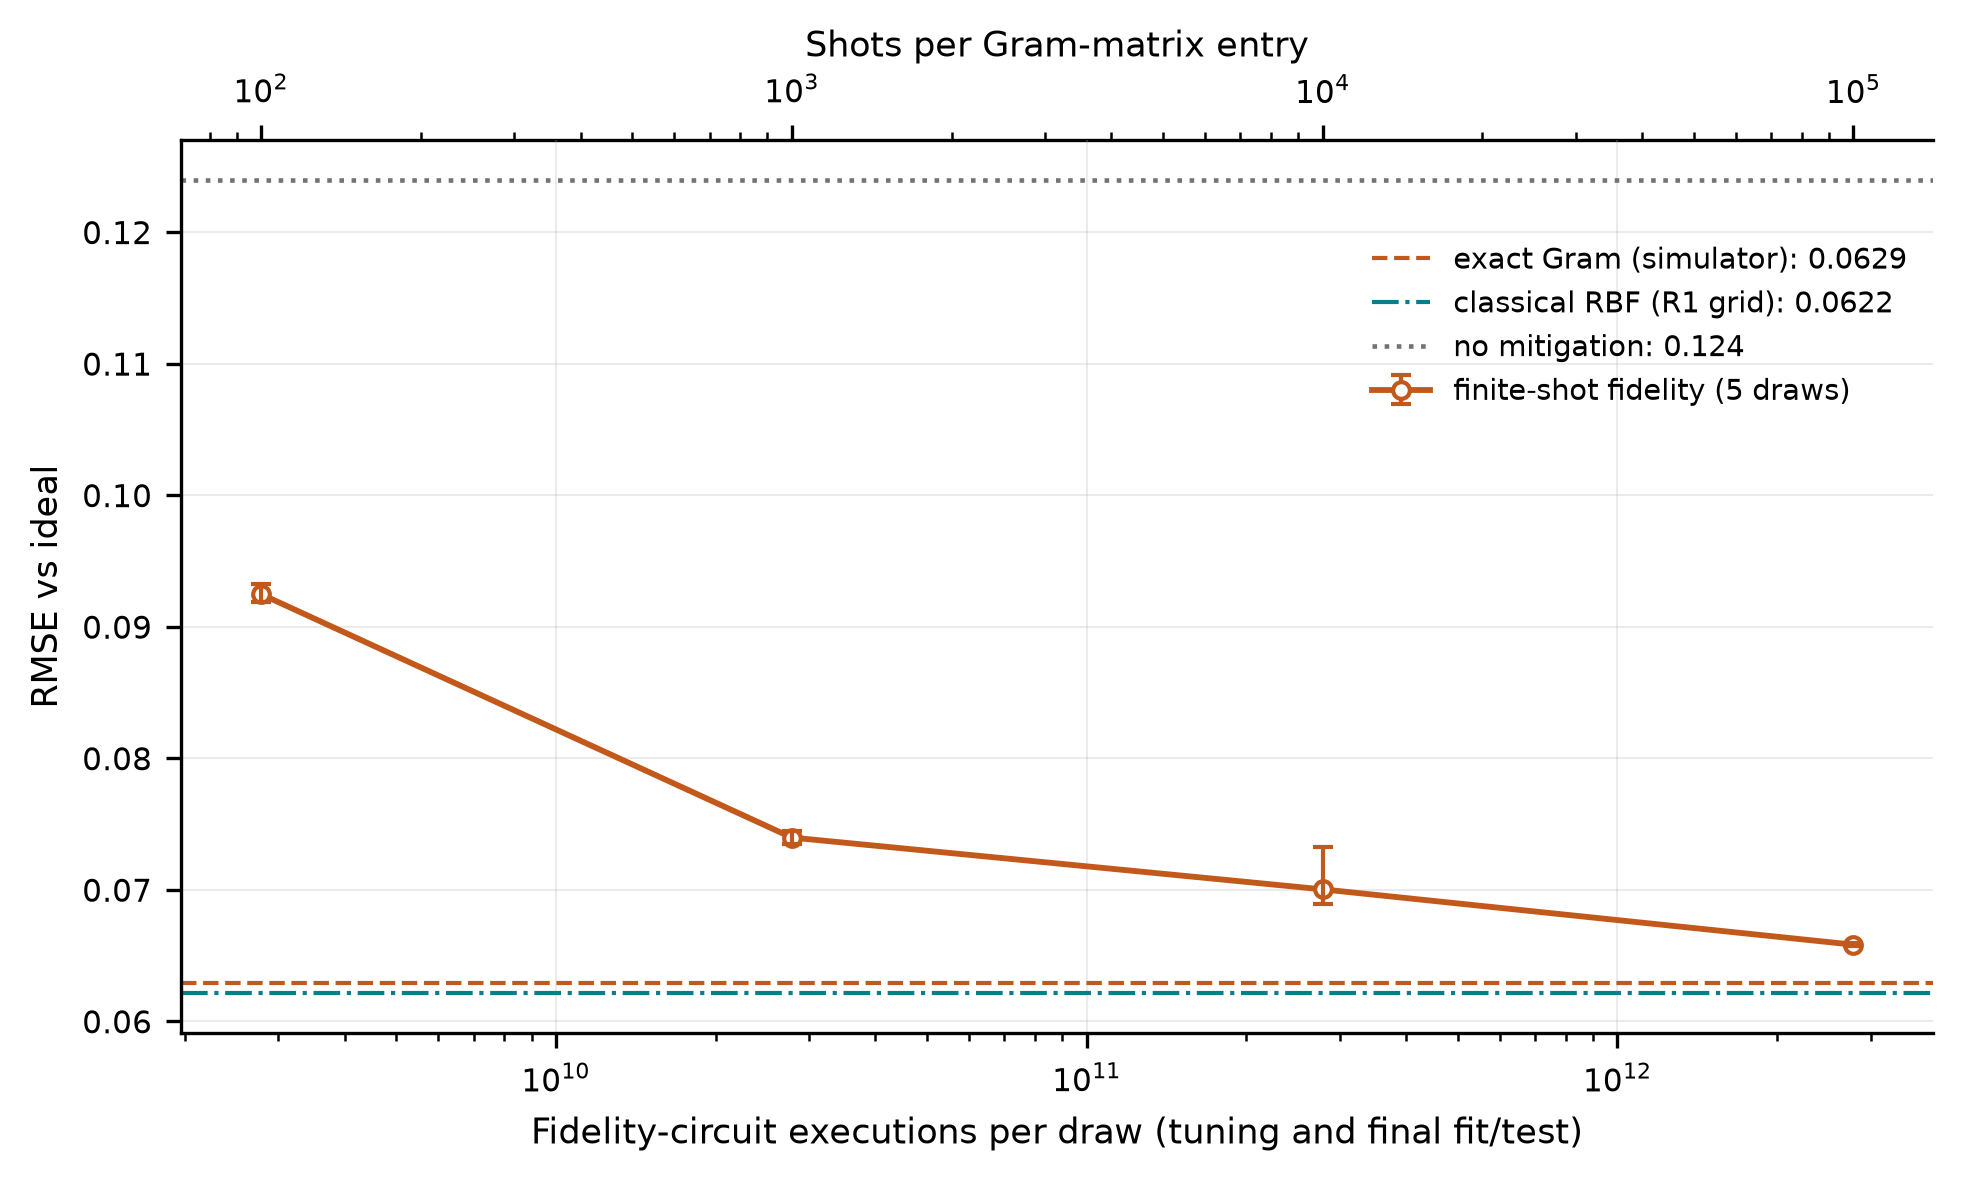
\includegraphics[width=0.82\textwidth]{figures/ch5/fig_ch5_shotkernel.png}
\caption[Shot-estimated quantum kernel against circuit executions]{Accuracy against the
total fidelity executions per draw for tuning and final fit/test. Error bars span the five
shot-noise draws. The RBF reference uses the same holdout with its R1 tuning grid.}
\label{fig:ch5_shotkernel}
\end{figure}

Table~\ref{tab:ch5_shotkernel} lists the accuracy and acquisition counts at each budget,
and Figure~\ref{fig:ch5_shotkernel} plots accuracy against total fidelity executions.
Mean RMSE declines at each tested increase in the shot budget. At the largest tested budget of $10^5$ shots per entry,
mean RMSE is $0.0658$ against $0.0629$ for the exact-Gram control,
a difference of $+0.0029$.
The simulated acquisition counts are $2.78\times 10^{12}$ fidelity executions to
tune, fit and test the model on this split and $3.15\times 10^{8}$ additional
executions for one subsequent prediction. The shared feature measurements
require $12{,}288$ executions per input row and are counted separately. The RBF fit
provides a cost reference with RMSE $0.0622$ and uses classical computation
for its kernel entries.

The penalty diagnostic compares the primary 12-point grid with a
nested 23-point grid on the same shot draws and folds. Both select $\alpha$
using grouped validation. The budget-wise mean RMSE difference (23-point $-$ 12-point) ranges from $-0.0008$ to $+0.0000$. The grid comparison is recorded in
\texttt{results/shot\_kernel\_alpha\_diagnosis.csv}.

\section{Matched kernels across both noise regimes}
\label{sec:ch5_realistic_summary}

Table~\ref{tab:ch5_kernelcompare} reports the direct RBF and fidelity
comparison across ten grouped holdouts of the reference pool for each setting.
The same training circuits, held-out circuits and candidate count are used
for both models in each holdout. These counts describe split sensitivity on fixed simulated datasets.
Section~\ref{sec:ch5_folding_seeds} compares the kernels across independent
circuit pools and shot draws.

\begin{table}[htbp]
\centering
\caption{Matched kernel comparison across the two noise regimes. RMSE is mean
$\pm$ SD over ten holdouts. The last three columns count paired circuit-bootstrap
intervals that favour RBF, favour fidelity or include zero.}
\label{tab:ch5_kernelcompare}
\small
\begin{tabular}{lccrrr}
\toprule
Setting & RBF RMSE & Fidelity RMSE & RBF & Fidelity & Includes 0 \\
\midrule
Idealised & $0.0416\pm0.0011$ & $0.0426\pm0.0012$ & 9 & 0 & 1 \\
Realistic, param. & $0.0638\pm0.0019$ & $0.0640\pm0.0019$ & 5 & 0 & 5 \\
Realistic, folding & $0.0771\pm0.0042$ & $0.0776\pm0.0043$ & 6 & 0 & 4 \\
Reset, param. & $0.0532\pm0.0008$ & $0.0533\pm0.0008$ & 2 & 1 & 7 \\
Reset, folding & $0.0571\pm0.0006$ & $0.0571\pm0.0006$ & 3 & 0 & 7 \\
\bottomrule
\end{tabular}
\end{table}

Both kernels have lower RMSE than folded linear ZNE in all ten
repeated holdouts for both the production and reset conditions, with
paired intervals excluding zero. The direct kernel comparison favours
RBF in six production holdouts and three reset holdouts under folding.

With shot-estimated entries, the fidelity kernel reaches $0.0658$ RMSE on the
parameter-scaled random holdout at $10^5$ shots per entry, against $0.0622$ for
RBF (Section~\ref{sec:ch5_shotkernel}). Finite fidelity also requires overlap measurements for the train and held-out
blocks, whereas RBF computes similarities from the shared observable features.

\end{document}
